\section{Overview: High-Level Components and Interactions}
\label{sec: overview}
In this section, a general description of the architecture of the S\&C system is provided.
The main architectural styles to be followed are:
\begin{itemize}
    \item \textbf{Client-Server Architecture:} This architecture was chosen for its simplicity and efficiency in managing user interactions and business logic. It is also scalable, as servers can be replicated and distributed to handle increasing user loads.
    \item \textbf{4-Tier Architecture:} The tier architecture and the number of levels are a natural consequence of the subdivision of functionalities across distinct layers, as it will be shown in the \hyperref[sec: deployment_view]{\uline{Deployment View}}. This approach supports a clear separation of concerns, ensuring each tier is responsible for a specific aspect of the system’s operation. This architecture enhances scalability, modularity and fault tolerance, separating each layer, and allows the system to adapt dynamically to workload demands while maintaining high availability and performance.
    \item \textbf{Microservices:} The system's functionalities have been split into separated microservices, each with its own dedicated database. This decision comes with plenty of benefits: for instance, it allows the achievement of better separation of concerns and decoupling between the functionalities offered, which consequently makes it possible to implement them in parallel and also to accomplish graceful degradation of the system in case of failures. Moreover, it enables different deployment strategies, such as containerization, enhancing system scalability.
    \item \textbf{REST - Representational State Transfer:} The designed microservices expose interfaces based on a REST API to communicate both with each other and the outside world. This decision allows to hide underlying technical aspects of the services since the communication is achieved through a technology-neutral protocol.
\end{itemize}

\newpage

\section{Component View}
\label{sec: component_view}

In this section, the main components of the S\&C system are outlined, with an accurate description of what each of them aims to accomplish. Every component is approximately derived from one of the product functions discussed in Section 2.2 of the RASD. Further, components are grouped together by affinity in high-level "macro-categories" to form microservices, obtaining what is usually referred to as "bounded contexts" in Domain-Driven Development (DDD). Components also expose interfaces with methods to be invoked from external entities and communicate with some databases.

\subsection{Component Diagram}
\label{subsec:component_diagram}
\begin{figure} [H]
    \begin{center}
        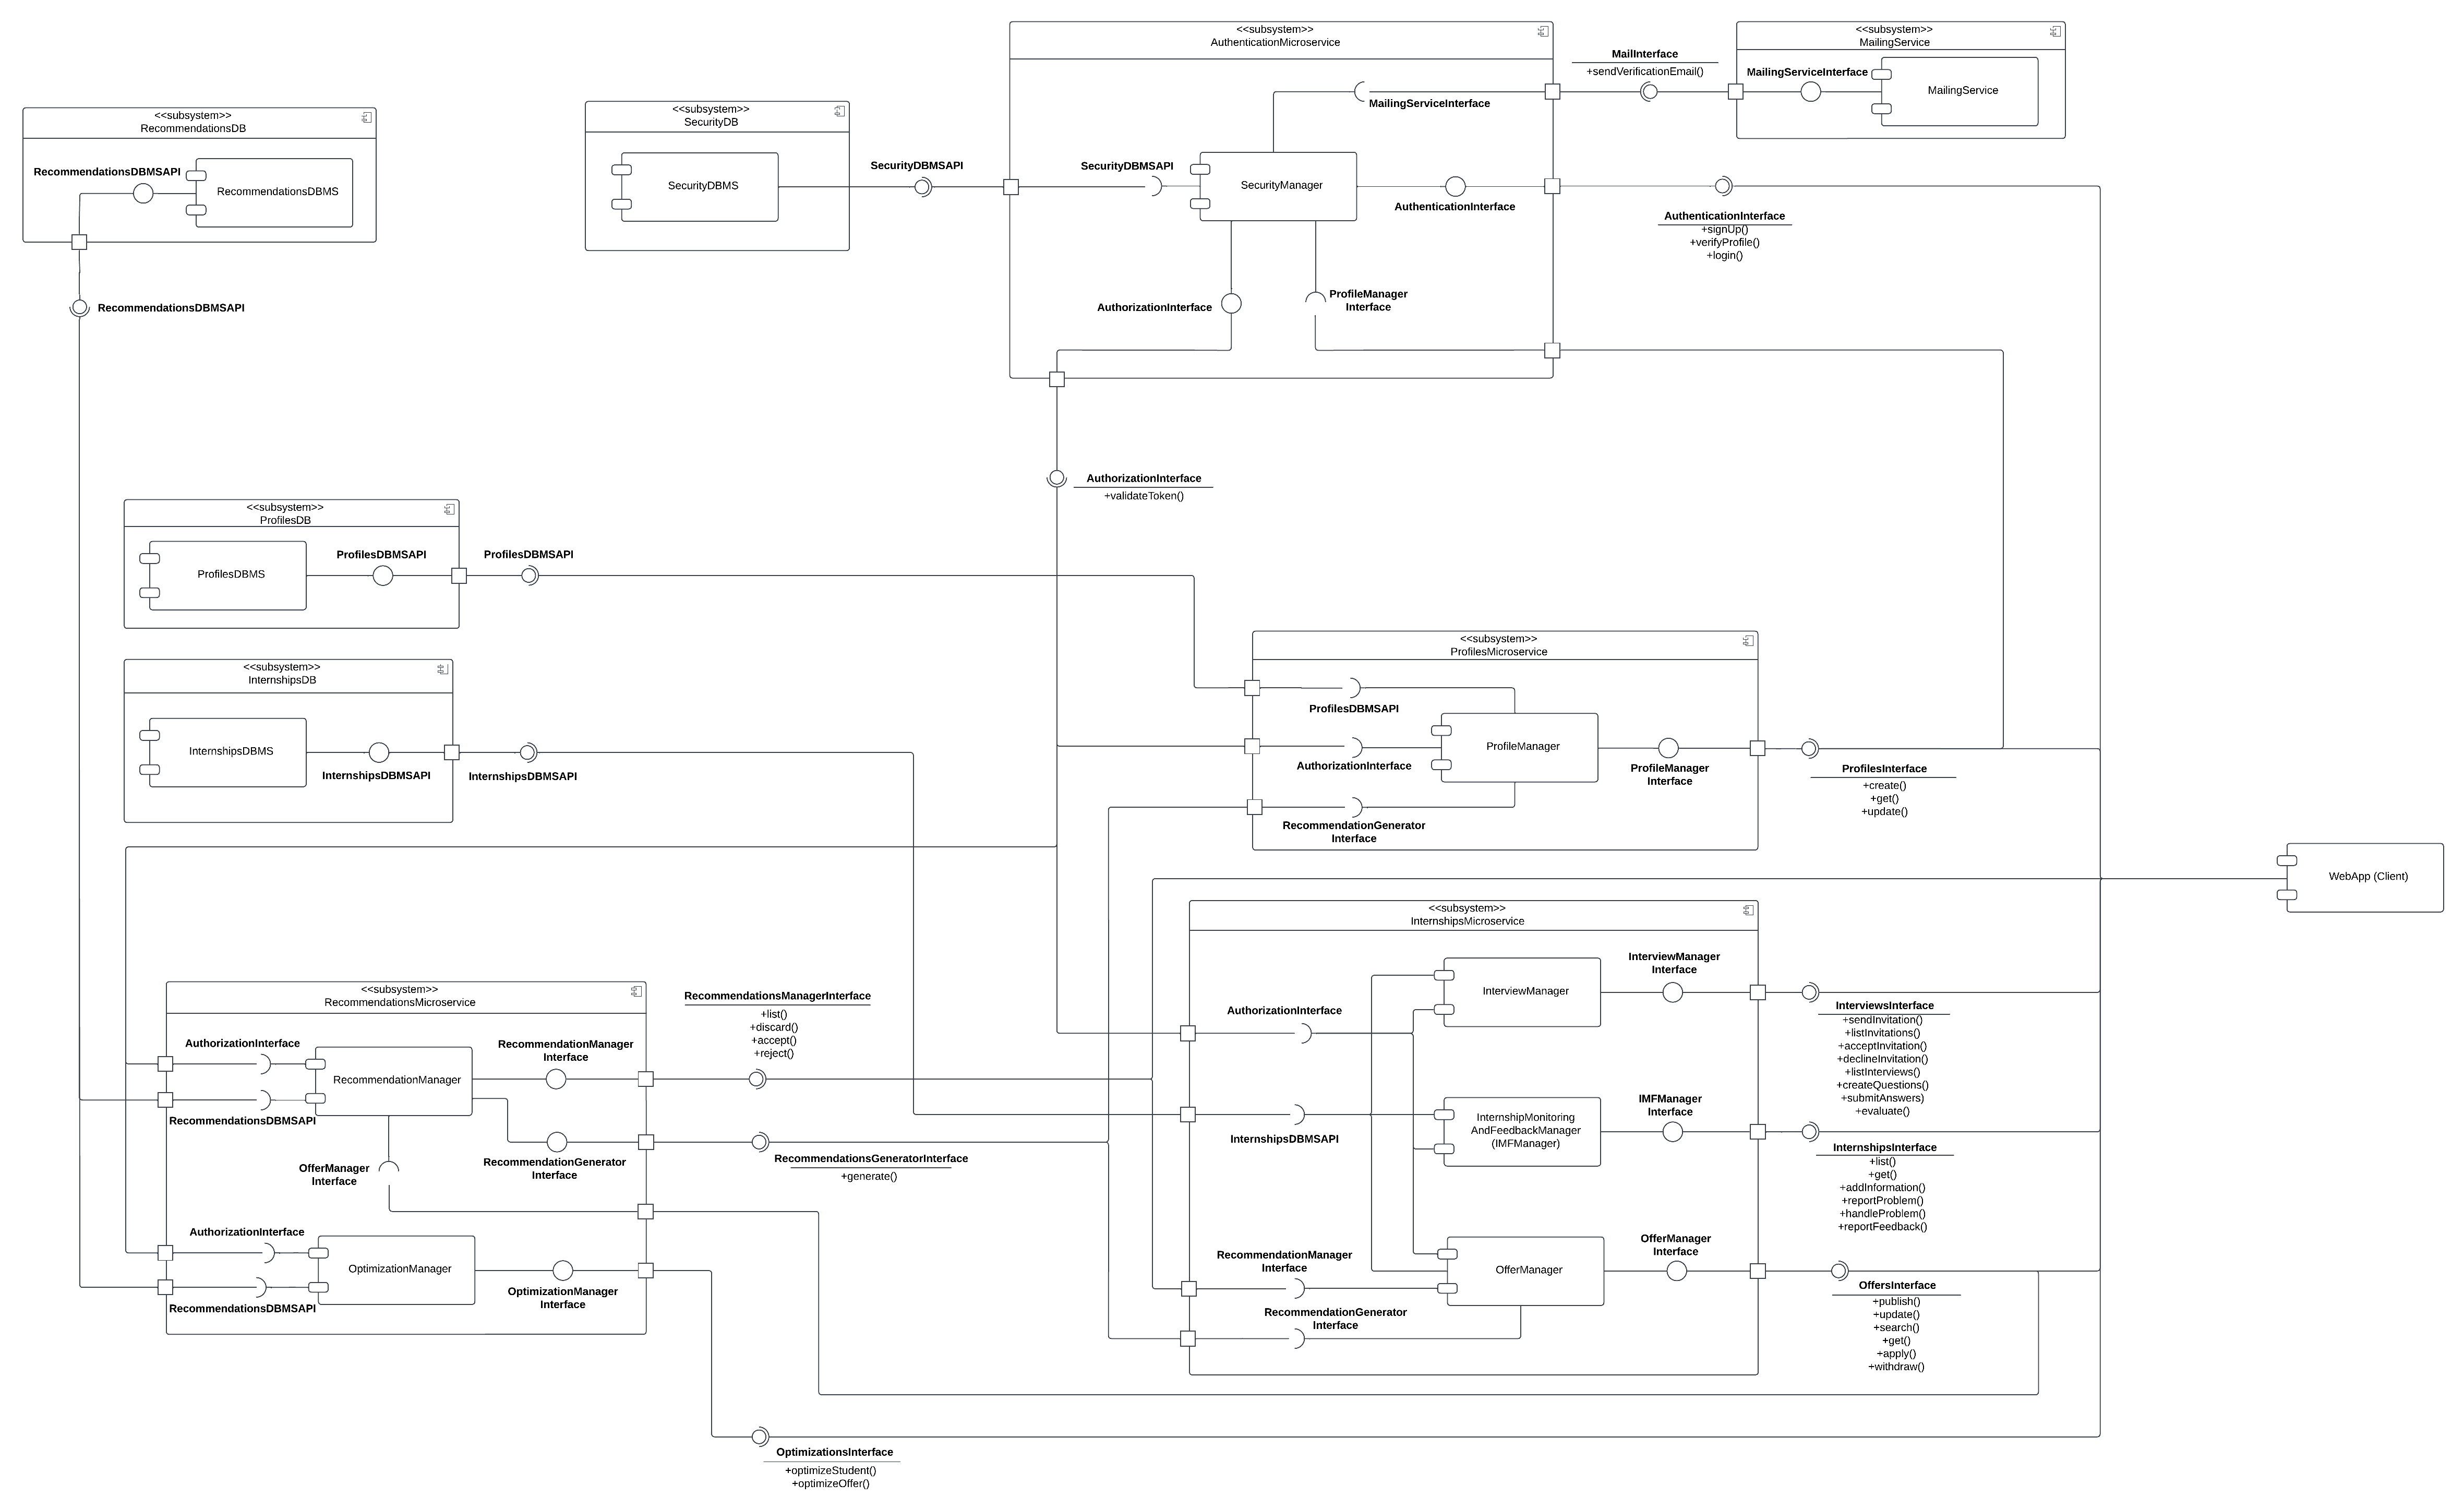
\includegraphics[width=0.95\linewidth]{LaTeXCode/images/ComponentDiagram/component_view.png}
        \caption{Component diagram of the S\&C system.}
        \label{fig:component_diagram}
    \end{center}
\end{figure}

\subsection{Components Description}
\label{subsec:components_description}

Each of the following components shall be thought of as a collection of simpler units that closely interact together to provide the offered functionalities. Specification of these units and how they form the component as a whole is left to the single teams or developers, as it is not binding towards the overall architecture of the system (given that every component must still fulfill the outlined expectations).

\begin{enumerate}
    \item \textbf{SecurityManager:} This component handles user authentication and registration processes for Students, Companies, and Universities. It manages the creation of new accounts by validating the provided information and communicating with the ProfileManager, and it also interacts with the MailingService to verify user identities. Additionally, it manages secure login operations, ensuring that only authenticated users can access the platform, and is used by other components to verify that users have the necessary authorization to execute the incoming requests.
    \item \textbf{MailingService:} This component handles the email communications needed for the ongoing account verification processes. It implements the mail server functionalities needed to send verification emails to users during the sign-up phase, each containing a link that shall be clicked to complete the registration process.
    \item \textbf{ProfileManager:} This component handles the operations required to view and update user profiles. For students, sign-ups or updates to relevant details initiate the generation of new recommendations by interacting with the RecommendationManager, aimed either at them or at some Companies, ensuring they both remain aligned with current opportunities.
    \item \textbf{OfferManager:} This component manages the lifecycle of internship offers within the platform. It provides companies with tools to create, update, withdraw and manage their internship announcements. When creating an offer, the OfferManager automatically extracts the relevant keywords to be applied to the offer from the description provided. The component also integrates advanced filtering mechanisms to allow students to search efficiently for relevant opportunities and view them. Moreover, the OfferManager facilitates interactions between students and companies by managing applications and allowing them to keep the status of offers up-to-date. As for the ProfileManager, this component interacts with the RecommendationManager to generate new recommendations when creating or updating relevant details of offers.
    \item \textbf{InterviewManager:} This component facilitates and manages the whole interview process between students and companies. It provides tools for scheduling, conducting, monitoring and evaluating interviews. The component ensures easy communication between the parties and handles the creation, delivery and management of interview invitations. Additionally, it records evaluations and updates the status of candidates in the selection process, easing the transition from interviews to final decisions.
    \item \textbf{InternshipMonitoringAndFeedbackManager (IMFM):} This component manages the monitoring, complaining and feedback processes for internships. It enables students and companies to provide updates and view detailed information about ongoing internships they are participating in. It also allows parties to report issues encountered during internships, forwarding these reports to the university for resolution. At the conclusion of an internship, the component facilitates the collection of feedback from both students and companies, so that this information can be used in the future to enhance the recommendation algorithms and ensure a continuous improvement of the system.
    \item \textbf{RecommendationManager:} This component handles the operations needed to generate and manage recommendations. It identifies internship recommendations for students and student recommendations for companies by performing graph analyses on a graph database storing the relationships between students, companies, offers, skills and various feedback expressed through time: specifically, the RecommendationManager detects links between the keywords associated with students' resumes and offers published, and can also perform more complex queries which statistically identify relationships between profiles, preferences and past histories of all users on the platform, by means of collaborative filtering and content-based filtering. Last, but not least, this component also allows both of them to view and act on their received recommendations.
    \item \textbf{OptimizationManager:} This component manages the operations needed to generate personalized suggestions to improve user content. It relies on a Large Language Model (LLM) that has been properly fine-tuned to identify enhancements to be applied to students' profiles and offers' descriptions to make them more appealing and increase their chances of being selected. The OptimizationManager also takes into account the opportunities (students and offers) currently available on the platform by feeding to the LLM some aggregated data resulting from whole-graph analyses, so that it can provide suggestions that are customized for the current situation.
    \item \textbf{SecurityDBMS, ProfilesDBMS, InternshipsDBMS:} relational DBMSs that store data respectively about account credentials, profiles information and internship information.
    \item \textbf{RecommendationsDBMS:} graph DBMS that stores data about the relationships between users, skills, internships, recommendations and useful feedback in order to identify new recommendations by simple skill keyword searching or statistical whole-graph analyses.
\end{enumerate}

\newpage

\section{Deployment View}
\label{sec: deployment_view}

The system is deployed as a distributed microservices architecture leveraging containerization and orchestration to achieve high scalability, resiliency and modularity. Each layer has distinct responsibilities and is deployed across a collection of servers to guarantee replication and fault tolerance.

\begin{itemize}
    \item \textbf{Presentation Layer:} represents the client in a traditional client-server architecture. Users interact with the system via a web application running in their browser.
    \item \textbf{Application Layer:} hosts containerized microservices that provide all business functionalities.
    The deployment diagram illustrates a possible allocation of these containers across the servers available to this layer. The actual number of microservice instances and their distribution during runtime are dynamically determined by the container orchestration platform based on workload demands. This ensures optimal resource utilization and adaptability to varying request volumes.
    \item \textbf{Service Management Layer:} responsible for managing the orchestration of microservices and auxiliary services. This layer includes the mailing service used during the registration process, the Data Layer Load Balancer, which manages the distribution of requests to database replicas in the Data Layer, and the Replication-Consistency Middleware, which handles data replication and consistency.
    \item \textbf{Data Layer:} manages persistent data storage using replicated databases to ensure fault tolerance and performance optimization. Data replicas are statically allocated, in order to implement strategic business decisions about scalability and geographic allocation manually, and the load balancer in the Service Management Layer ensures requests are distributed evenly across these replicas.
\end{itemize}

Communication between the components relies on REST APIs (HTTPS), with TCP/IP for lower-level communication, especially with the Service Management Layer and with the Data Layer.

\begin{figure} [H]
    \begin{center}
        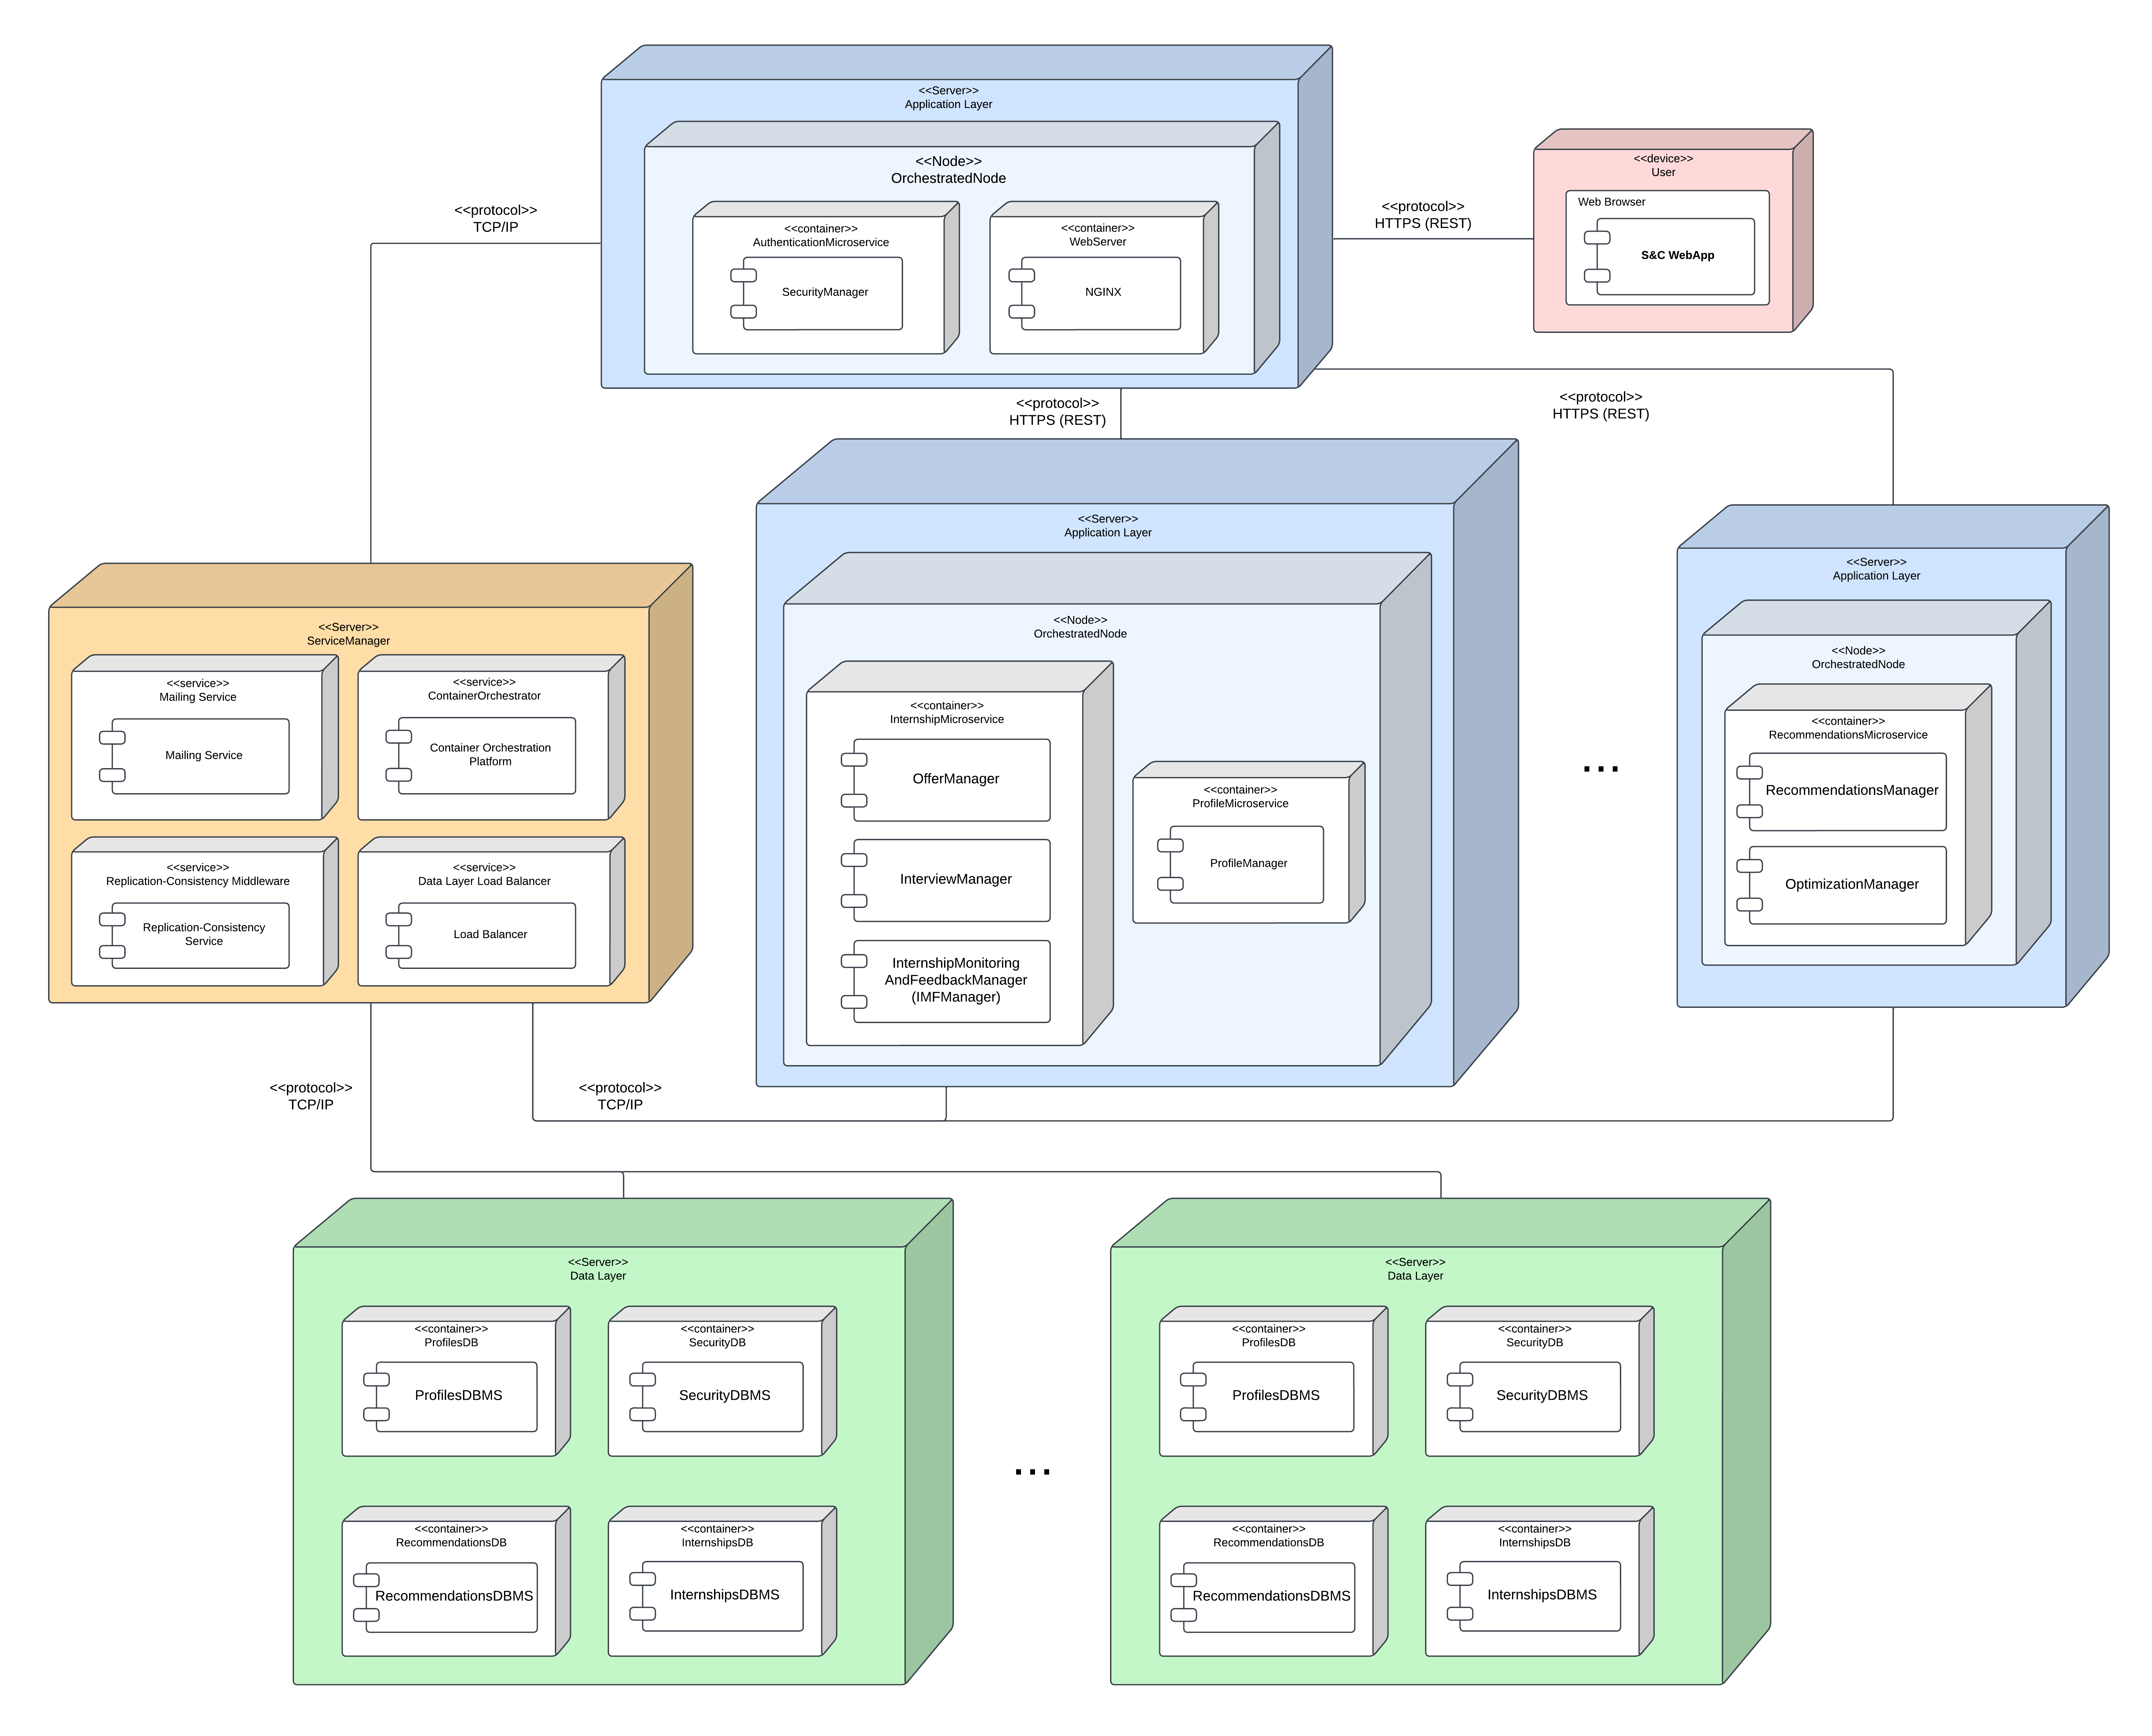
\includegraphics[width=0.95\linewidth]{LaTeXCode/images/DeploymentDiagram/deployment_view.png}
        \caption{UML Deployment Diagram.}
        \label{fig: deployment_diagram}
    \end{center}
\end{figure}

\subsection{Detailed Layer Decisions}
\label{subsec: layer_description}

\paragraph{Web Server}
The entry point of the application is NGINX, a web server deployed in a container acting as a reverse proxy, hosting all API endpoints, acting as an API Gateway and forwarding the requests from the user layer to the appropriate microservices in the application layer. 
The component gatekeeps all traffic to microservices and collaborates with the SecurityManager in order to provide authentication and authorization mechanisms.
Internally, it also performs load balancing of the incoming requests and URL rewriting a redirection. 
It simplifies routing logic and improves the security of the system by exposing a single public endpoint.

\paragraph{Scalability}
Each microservice and DBMS runs in an isolated container, enabling independent scaling. The container orchestrator dynamically adjusts the number of containers based on resource consumption or incoming traffic, and replication in the Data Layer improves read performance by distributing queries across replicas.

\paragraph{Resiliency}
The container orchestration platform manages failover and automatically restarts containers in case of crashes.
Data replication ensures availability, even in the event of server failure and the Data Layer Load Balancer prevents overloading by evenly distributing requests.

\paragraph{Orchestration Platform Considerations}
A specific Container Orchestration Technology is not specified, even if ideally it would be preferable to use Kubernetes and deploy the containers with Docker, since they are the most widely adopted platforms and are well known to system administrators, simplifying their use for all the people involved in deploying and managing the infrastructure.
In particular, the orchestrator offers many useful functionalities in the context of our architecture, such as automatic scaling, monitoring, networking and server-side service discovery, lightening the burden of managing such aspects.
In the server-side discovery method, services are registered with an API server (if Kubernetes is chosen, called Kubernetes API Server), which acts as a central registry for services. Clients then query the API server to discover the available services, which are dynamically deployed and for this reason real addresses may change. The API server responds with a list of available microservices and their corresponding endpoints. When the reverse proxy makes a network request for a service, the Orchestration Platform routes the request to the appropriate endpoint using the information stored. While doing this, the orchestration platform also manages load balancing among the available microservices.

\paragraph{Replication and Data Consistency}
The Data Layer adopts a Multi-Leader Replication protocol to maintain consistency across replicas, accommodating the geographical distribution of data nodes. This approach enables multiple leaders to handle write operations concurrently, reducing latency and ensuring high availability.
In this setup, write operations can be performed on any leader node. Changes are then propagated asynchronously to other leaders and replicas, ensuring eventual consistency across the system.
Read operations are distributed across multiple replicas to optimize performance and handle high query volumes effectively.
This replication model provides enhanced fault tolerance, as the failure of a single leader does not disrupt write operations. However, potential conflicts from concurrent writes have to be managed using conflict resolution strategies, ensuring data integrity across all replicas.

\newpage

\section{Component Interfaces}
\label{sec: component_interfaces}
In this section the component interfaces defined are described, highlighting for each one the expected inputs and outputs.

\subsection{REST API Endpoints}
Each microservice of the system exposes one or more interfaces, which are the resource endpoints of the defined REST API. The Service Orchestrator is responsible for carrying out the Service Discovery process among the physical servers, as it is the one that knows how microservices are deployed on the different machines at every instant, and can thus route the requests aimed at the specific resources to the correct location for the corresponding microservice.
The structure of an API request directed to a microservice of the system must adhere to the following structure:

\texttt{https://DOMAIN/api/VERSION/INTERFACE/FUNCTION}

In particular:
\begin{itemize}
    \item The communication protocol must be HTTPS.
    \item \texttt{DOMAIN} is the domain name of the S\&C system.
    \item \texttt{/api/} is just syntactic sugar to highlight that the request is aimed at an API resource.
    \item \texttt{VERSION} is the version of the API to be addressed (for compatibility purposes).
    \item \texttt{INTERFACE} is the first-level hierarchy, indicating the specific interface to be addressed (not the actual microservices, as they could expose more than one interface): every interface keeps the same name indicated in the Component View in \hyperref[fig:component_diagram]{\protect\uline{Section 2.2.1}}, but without the final "Interface" keyword.
    \item \texttt{FUNCTION} is the API procedure of the specified interface that is being requested.
\end{itemize}

The following is a list of all the API endpoints, grouped by interface: for each one, the expected input parameters, responses\footnote{Both here and in the Sequence Diagrams in \hyperref[sec:runtime_view]{\protect\uline{Section 2.5}}, all \textbf{400 Bad Request} responses for requests about nonexisting resources (such as invalid IDs) are omitted for brevity. The same goes for \textbf{401 Unauthorized} responses, generated and forwarded by the SecurityManager upon denial resulting from calls to its \texttt{/validateToken} endpoint: even if omitted at the moment, such calls shall be present in the implementation code whenever a request that involves access to any protected resource is received and whenever access authorization of the requestor needs to be verified.} (with eventual important headers), and output values are listed. For additional security, the endpoints must always be invoked through the HTTPS POST method: input parameters and eventual output values are always provided respectively in the body of the request and the response, and both must be in standard JSON format.

\subsubsection*{/authentication}
\begin{itemize}
    \item \texttt{/signUp} \\
        \textit{parameters:} \{ email: String, password: String, accountType: Enum(Student, Company, University) \} \\
        \textit{responses:}
        \begin{itemize}
            \item \textbf{303 See Other:} \\ 
            header: "Location: loginPage", \\
            body: \{ cause: Enum(alreadyRegistered, emailSent) \}
            \item \textbf{400 Bad Request:} \\
            body: \{ error: Enum(missingFields, invalidPassword) \}
        \end{itemize}
    \item \texttt{/verifyProfile}\footnote{As an exception, this is the only endpoint to be accessed through a GET request, as it is intended to be invoked by clicking the link in the verification email.} \\
        \textit{parameters:} \{ userID: int \} \\
        \textit{responses:} 
        \begin{itemize}
            \item \textbf{308 Permanent Redirect:} \\
            header: "Location: updateProfilePage" \\
            body: \{ cause: Enum(profileVerified) \}
        \end{itemize}
    \item \texttt{/login} \\
        \textit{parameters:} \{ username: String, password: String \footnote{Note that it is not the actual password, but only its hash value.} \}\\
        \textit{responses:}
        \begin{itemize}
            \item \textbf{308 Permanent Redirect:} \\
            header: "Location: dashboardPage" \\
            body: \{ cause: Enum(successfulLogin), token: String \}
            \item \textbf{308 Permanent Redirect:} \\
            header: "Location: updateProfilePage" \\
            body: \{ cause: Enum(incompleteProfile), token: String \}
            \item \textbf{400 Bad Request:} \\
            body: \{ error: Enum(wrongCredentials, unverifiedAccount) \}
        \end{itemize}
\end{itemize}

\subsubsection*{/mail}
\begin{itemize}
    \item \texttt{/sendVerificationEmail} \\
        \textit{parameters:} \{ email: String, confirmationLink: String \} \\
        \textit{responses:}
        \begin{itemize}
            \item \textbf{204 No Content}
        \end{itemize}
\end{itemize}

\subsubsection*{/authorization}
\begin{itemize}
    \item \texttt{/validateToken} \\
        \textit{parameters:} \{ token : String \} \\
        \textit{responses:}
        \begin{itemize}
            \item \textbf{200 OK:} \\
            body: \{ authorized: true \}
            \item \textbf{401 Unauthorized:} \\
            body: \{ authorized: false \}
        \end{itemize}
\end{itemize}

\subsubsection*{/profiles}
\begin{itemize}
    \item \texttt{/create} \\
        \textit{parameters:} \{ userID: int, user: User \} \\
        \textit{responses:}
        \begin{itemize}
            \item \textbf{204 No Content}
        \end{itemize}
    \item \texttt{/get} \\
        \textit{parameters:} \{ userID: int \} \\
        \textit{responses:}
        \begin{itemize}
            \item \textbf{200 OK:} \\
            body: \{ user: User \}
            \item \textbf{400 Bad Request:} \\
            body: \{ cause: Enum(invalidUser) \}
        \end{itemize}
    \item \texttt{/update} \\
        \textit{parameters:} \{ userID: int, user: User \} \\
        \textit{responses:}
        \begin{itemize}
            \item \textbf{200 OK:} \\
            body: \{ popup: Enum(profileUpdated), user: User \}
            \item \textbf{400 Bad Request:} \\
            body: \{ cause: Enum(missingFields) \}
        \end{itemize}
\end{itemize}

\subsubsection*{/offers}
\begin{itemize}
    \item \texttt{/publish} \\
        \textit{parameters:} \{ companyID: int, offer: Offer \} \\
        \textit{responses:}
        \begin{itemize}
            \item \textbf{307 Temporary Redirect:} \\
            header: "Location: offerPage" \\
            body: \{ popup: Enum(offerPublished), offerID: int \}
            \item \textbf{400 Bad Request:} \\
            body: \{ cause: Enum(missingFields, nonCompliantInformation) \}
        \end{itemize}
    \item \texttt{/update} \\
        \textit{parameters:} \{ companyID: int, offerID: int, offer: Offer \} \\
        \textit{responses:}
        \begin{itemize}
            \item \textbf{200 OK:} \\
            body:  \{ popup: Enum(offerUpdated), offer: Offer \}
            \item \textbf{400 Bad Request:} \\
            body: \{ cause: Enum(missingFields, nonCompliantInformation) \}
        \end{itemize}
    \item \texttt{/search} \\
        \textit{parameters:} \{ filters: [ filter: Filter ] \} \\
        \textit{responses:}
        \begin{itemize}
            \item \textbf{200 OK:} \\
            body: \{ offersList: [ offer: Offer ] \}
        \end{itemize}
    \item \texttt{/get} \\
        \textit{parameters:} \{ offerID: int \} \\
        \textit{responses:}
        \begin{itemize}
            \item \textbf{200 OK:} \\
            body: \{ offer: Offer \}
        \end{itemize}
    \item \texttt{/apply} \\
        \textit{parameters:} \{ studentID: int, offerID: int \} \\
        \textit{responses:}
        \begin{itemize}
            \item \textbf{200 OK:} \\
            body: \{ popup: Enum(applicationSubmitted) \}
            \item \textbf{400 Bad Request:} \\
            body: \{ cause: Enum(expiredDeadline) \}
        \end{itemize}
    \item \texttt{/withdraw} \\
        \textit{parameters:} \{ companyID: int, offerID: int \} \\
        \textit{responses:}
        \begin{itemize}
            \item \textbf{308 Permanent Redirect:} \\
            header: "Location: dashboardPage" \\
            body: \{ cause: Enum(successfulWithdrawal) \}
        \end{itemize}
\end{itemize}

\subsubsection*{/interviews}
\begin{itemize}
    \item \texttt{/sendInvitation} \\
        \textit{parameters:} \{ studentID: int, offerID: int, date: DateTime, type: Enum(inPerson, inPlatform), otherDetails: String \} \\
        \textit{responses:}
        \begin{itemize}
            \item \textbf{200 OK:} \\
            body: \{ popup: Enum(invitationSent) \}
        \end{itemize}
    \item \texttt{/listInvitations} \\
        \textit{parameters:} \{ userID: int\} \\
        \textit{responses:}
        \begin{itemize}
            \item \textbf{200 OK:} \\
            body: [ \{ offerID: int, offer: Offer, date: DateTime, type: Enum(inPerson, inPlatform), otherDetails: String \} ]
        \end{itemize}
    \item \texttt{/acceptInvitation} \\
        \textit{parameters:} \{ offerID: int, studentID: int \} \\
        \textit{responses:}
        \begin{itemize}
            \item \textbf{200 OK:} \\
            body: \{ popup: Enum(invitationAccepted) \}
        \end{itemize}
    \item \texttt{/declineInvitation} \\
        \textit{parameters:} \{ offerID: int, studentID: int, reason: String \} \\
        \textit{responses:}
        \begin{itemize}
            \item \textbf{200 OK:} \\
            body: \{ popup: Enum(invitationDeclined) \}
        \end{itemize}
    \item \texttt{/listInterviews} \\
        \textit{parameters:} \{ userID: int\} \\
        \textit{responses:}
        \begin{itemize}
            \item \textbf{200 OK:} \\
            body: [ \{ interviewID: int, interview: Interview \} ]
        \end{itemize}
    \item \texttt{/createQuestions} \\
        \textit{parameters:} \{ companyID: int, interviewsIDs: [ interviewID: int ], questions: [ content : String ] \} \\
        \textit{responses:}
        \begin{itemize}
            \item \textbf{200 OK:} \\
            body: \{ popup: Enum(questionsCreated), questions: [ \{ questionIDs: int, question: Question \} ] \}
        \end{itemize}
    \item \texttt{/submitAnswer} \\
        \textit{parameters:} \{ studentID: int, interviewID: int, questionID: int,  answer: String \} \\
        \textit{responses:}
        \begin{itemize}
            \item \textbf{200 OK:} \\
            body: \{ popup: Enum(answerSubmitted), answer: Answer \}
        \end{itemize}
    \item \texttt{/evaluate} \\
        \textit{parameters:} \{ studentID: int, offerID: int, status: Enum(Selected, Rejected), feedback: String \} \\
        \textit{responses:}
        \begin{itemize}
            \item \textbf{200 OK:} \\
            body: \{ popup: Enum(interviewEvaluated) \}
        \end{itemize}
\end{itemize}

\subsubsection*{/internships}
\begin{itemize}
    \item \texttt{/list} \\
        \textit{parameters:} \{ userID: int \} \\
        \textit{responses:}
        \begin{itemize}
            \item \textbf{200 OK:} \\
            body: [ \{ internshipID: int, internship: Internship \} ]
        \end{itemize}
    \item \texttt{/get} \\
        \textit{parameters:} \{ internshipID: int, userID: int \} \\
        \textit{responses:}
        \begin{itemize}
            \item \textbf{200 OK:} \\
            body: \{ internship: Internship \}
        \end{itemize}
    \item \texttt{/addInformation} \\
        \textit{parameters:} \{ internshipID: int, userID: int, information: String \} \\
        \textit{responses:}
        \begin{itemize}
            \item \textbf{200 OK:} \\
            body: \{ popup: Enum(informationAdded) \}
        \end{itemize}
    \item \texttt{/reportProblem} \\
        \textit{parameters:} \{ internshipID: int, userID: int, problem: String \} \\
        \textit{responses:}
        \begin{itemize}
            \item \textbf{200 OK:} \\
            body: \{ popup: Enum(problemReported) \}
            \item \textbf{400 Bad Request:} \\
            body: \{ cause: Enum(missingFields) \}
        \end{itemize}
    \item \texttt{/handleProblem} \\
        \textit{parameters:} \{ internshipID: int, problemID: int, status: Enum(Unhandled, In Progress, Solved, Hidden) \} \\
        \textit{responses:}
        \begin{itemize}
            \item \textbf{200 OK:} \\
            body: \{ popup: Enum(statusUpdated), problemID: int, status: Enum(Unhandled, In Progress, Solved, Hidden) \}
        \end{itemize}
    \item \texttt{/reportFeedback} \\
        \textit{parameters:} \{ internshipID: int, userID: int, feedback: String \} \\
        \textit{responses:}
        \begin{itemize}
        \item \textbf{200 OK:} \\
            body: \{ popup: Enum(feedbackReported) \}
        \end{itemize}
\end{itemize}

\newpage

\subsubsection*{/recommendations/generator}
\begin{itemize}
    \item \texttt{/generate}\footnote{Calls to this API endpoint are overloaded, as the new or updated Student or Offer needs to be sent to the RecommendationManager, because changes might still not have been recorded in the RecommendationsDBMS because of eventual consistency.} \\
        \textit{parameters:} \{ studentID: int, student: Student \} \\
        \textit{responses:}
        \begin{itemize}
            \item \textbf{204 No Content}
        \end{itemize}
    \item \texttt{/generate}$^4$ \\
        \textit{parameters:} \{ offerID: int, offer: Offer \} \\
        \textit{responses:}
        \begin{itemize}
            \item \textbf{204 No Content}
        \end{itemize}
\end{itemize}

\subsubsection*{/recommendations/manager}
\begin{itemize}
    \item \texttt{/list} \\
        \textit{parameters:} \{ userID: int \} \\
        \textit{responses:}
        \begin{itemize}
            \item \textbf{200 OK:} \\
            body: \{ listOfRecommendations: [ recommendation: Recommendation ] \}
        \end{itemize}
    \item \texttt{/discard} \\
        \textit{parameters:} [ recommendationID: int ] \\
        \textit{responses:}
        \begin{itemize}
            \item \textbf{200 OK:} \\
            body: \{ popup: Enum(successfullyDiscarded) \}
        \end{itemize}
    \item \texttt{/accept} \\
        \textit{parameters:} [ recommendationID: int ] \\
        \textit{responses:}
        \begin{itemize}
            \item \textbf{200 OK:} \\
            body: \{ popup: Enum(successfullyAccepted) \}
        \end{itemize}
    \item \texttt{/reject} \\
        \textit{parameters:} [ recommendationID: int ] \\
        \textit{responses:}
        \begin{itemize}
            \item \textbf{200 OK:} \\
            body: \{ popup: Enum(successfullyRejected) \}
        \end{itemize}
\end{itemize}

\subsubsection*{/optimizations}
\begin{itemize}
    \item \texttt{/optimizeStudent} \\
        \textit{parameters:} \{ userID: int \} \\
        \textit{responses:}
        \begin{itemize}
            \item \textbf{200 OK:} \\
            body: \{ suggestedOptimizations: String \}
        \end{itemize}
    \item \texttt{/optimizeOffer} \\
        \textit{parameters:} \{ offerID: int \} \\
        \textit{responses:}
        \begin{itemize}
            \item \textbf{200 OK:} \\
            body: \{ suggestedOptimizations: String \}
        \end{itemize}
\end{itemize}

\subsection{Other Interfaces}

No additional interfaces are needed for the S\&C system, as no components inside a specific microservice ever need to communicate.

\newpage

\section{Runtime View}
\label{sec:runtime_view}%
In this section, the dynamic behavior of the S\&C system is portrayed. For each Use Case identified in Section 3.1 \textit{Use Cases and Activity Diagrams} of the RASD, the corresponding Sequence Diagram is provided, highlighting communication and messages exchanged between the components.
Once again, irrelevant details (such as: most client-side interactions between the User and the WebApp, e.g. form filling or negligible button clicking; call of most \texttt{get} functions of the API; extremely common operations such as calls to the \texttt{validateToken} function of the API) have been left out, as they would add further unnecessary complexity to the model, preventing a clear understanding of how components interact together.

\newcounter{uc}
\setcounter{uc}{1}
\newcommand{\cuc}{\theuc\stepcounter{uc}}

\subsubsection*{SD\cuc. Sign Up by a Student}
\label{subsubsec:signup_student_sd}
The Student clicks the "Sign Up" button on the sign up page and submits their data via the \texttt{.../api/v1/authentication/signUp/...} API endpoint. The request is forwarded to the \texttt{SecurityManager}, which validates the inputs and checks in the \texttt{SecurityDBMS} if the Student is already registered. If all checks succeed, it stores the Student data and calls the \texttt{MailingService} API to send a verification email to the specified email address through Simple Mail Transfer Protocol (SMTP). When the Student receives the email, if they click on the confirmation link within 24 hours, a call to the \texttt{.../api/v1/authentication/verifyProfile/...} API endpoint is made: the account is marked as verified in the \texttt{SecurityDBMS}, and the Student is redirected to the page for updating their profile, which takes place according to \hyperref[fig:update_profile_sd]{\protect\uline{SD5 - Update User Profile}}. If the timer for the verification instead expires, the account data is deleted from the \texttt{SecurityDBMS}.

\newpage

\begin{figure}[H]
    \begin{center}
         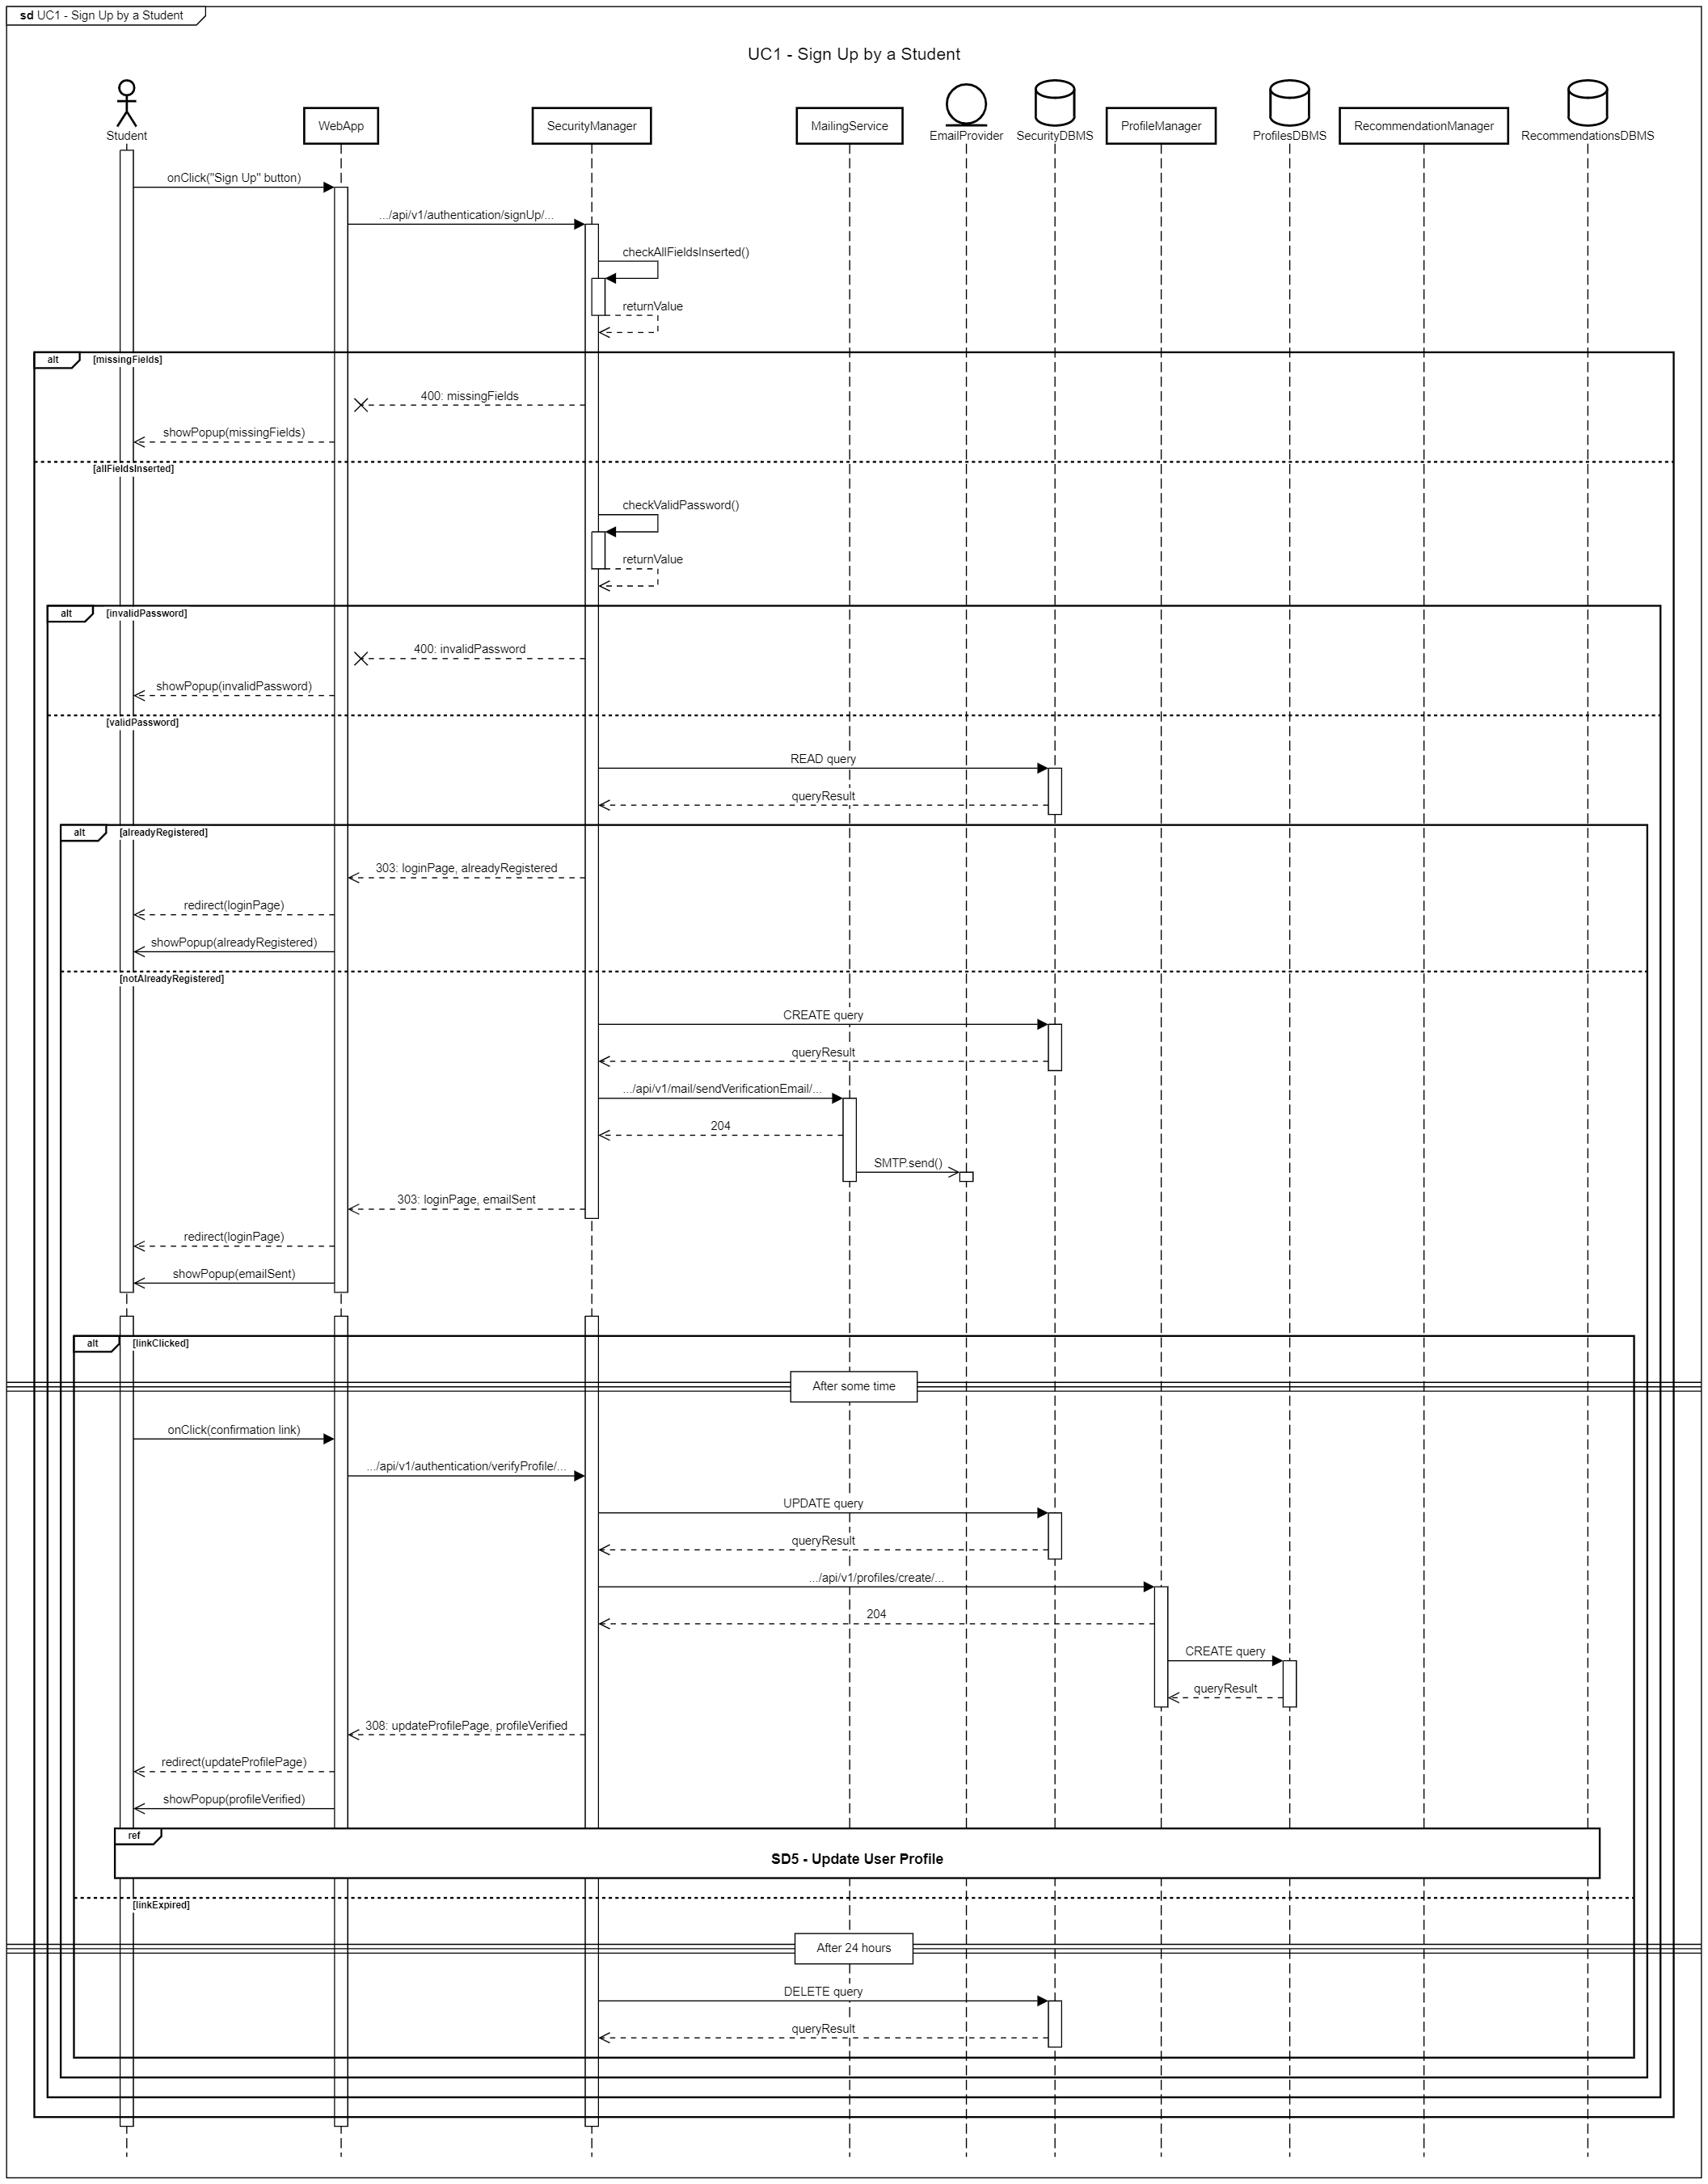
\includegraphics[width=1\linewidth]{LaTeXCode/images/SequenceDiagrams/UC1-sequenceDiagram.png}
         \caption{Sign Up by a Student}
         \label{fig:signup_student_sd}
     \end{center}
\end{figure}

\newpage

\subsubsection*{SD\cuc. Sign Up by a Company}
\label{subsubsec:signup_company_sd}
This Sequence Diagram is the same as the previous one, the only difference being that is is started by a Company and not by a Student.

\begin{figure}[H]
    \begin{center}
         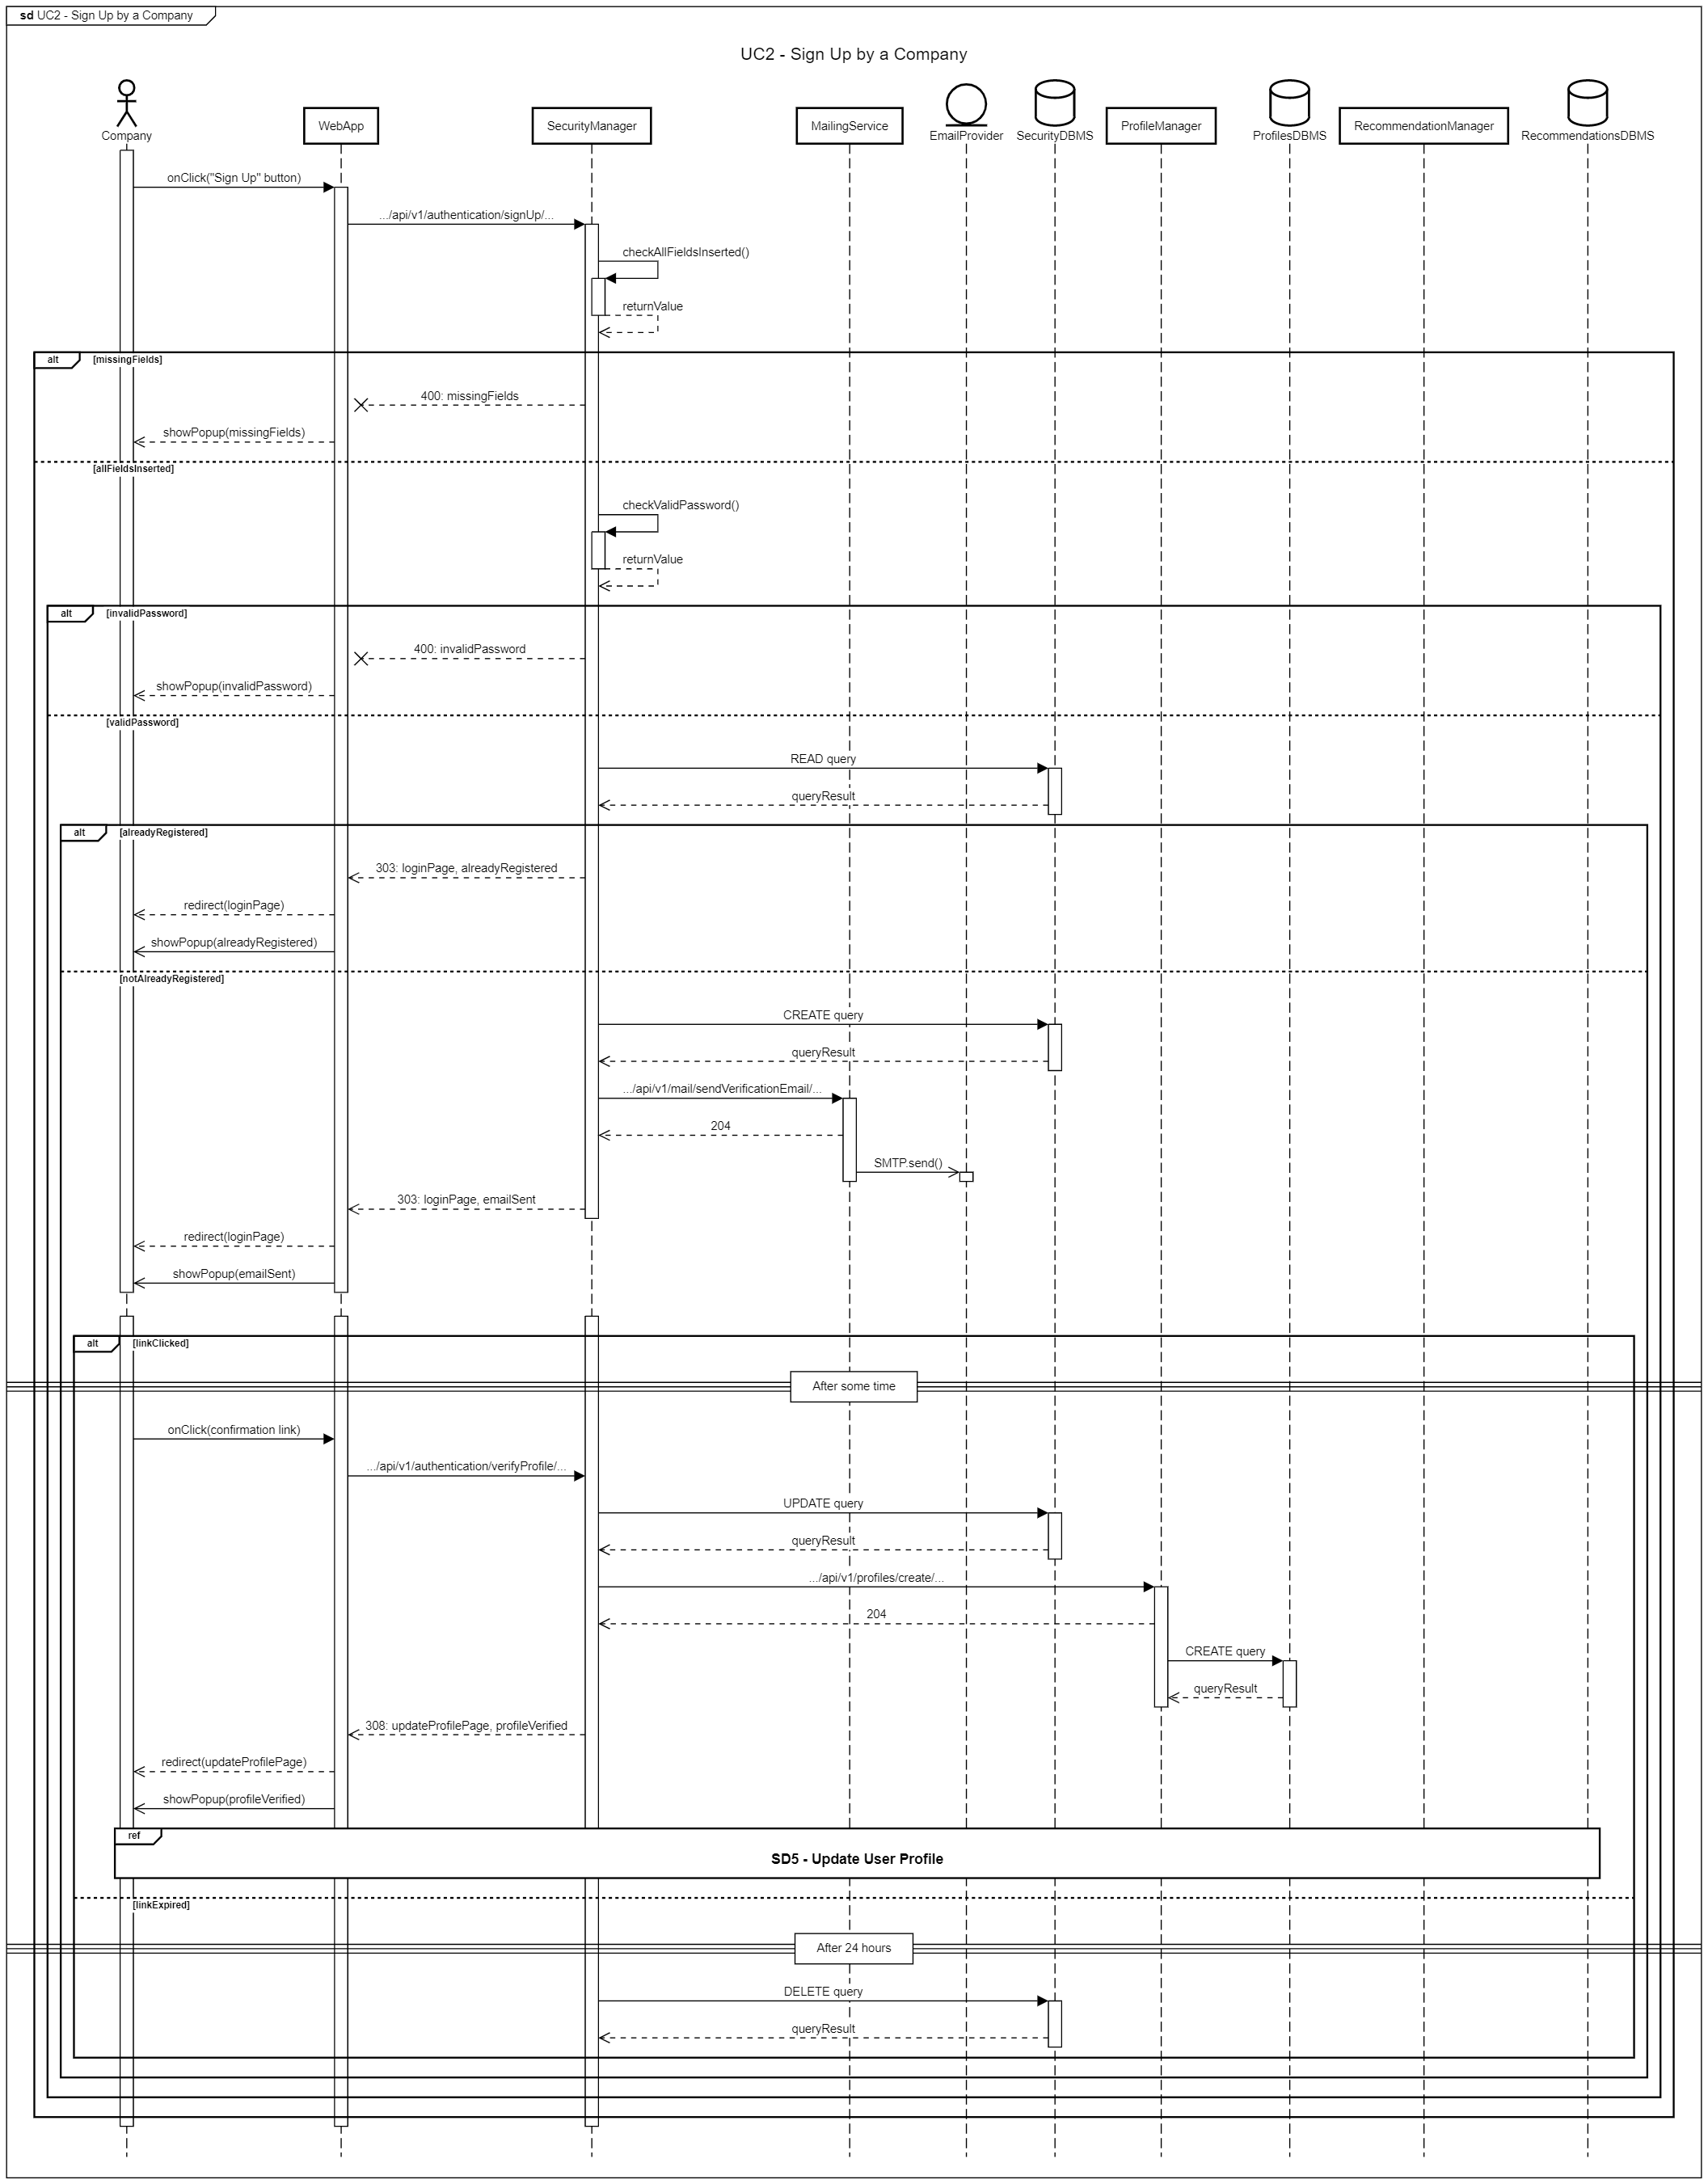
\includegraphics[width=0.9\linewidth]{LaTeXCode/images/SequenceDiagrams/UC2-sequenceDiagram.png}
         \caption{Sign Up by a Company}
         \label{fig:signup_company_sd}
     \end{center}
\end{figure}

\subsubsection*{SD\cuc. Sign Up by a University}
\label{subsubsec:signup_university_sd}
The same goes for this Sequence Diagram, which is in turn started by a University.

\begin{figure}[H]
    \begin{center}
         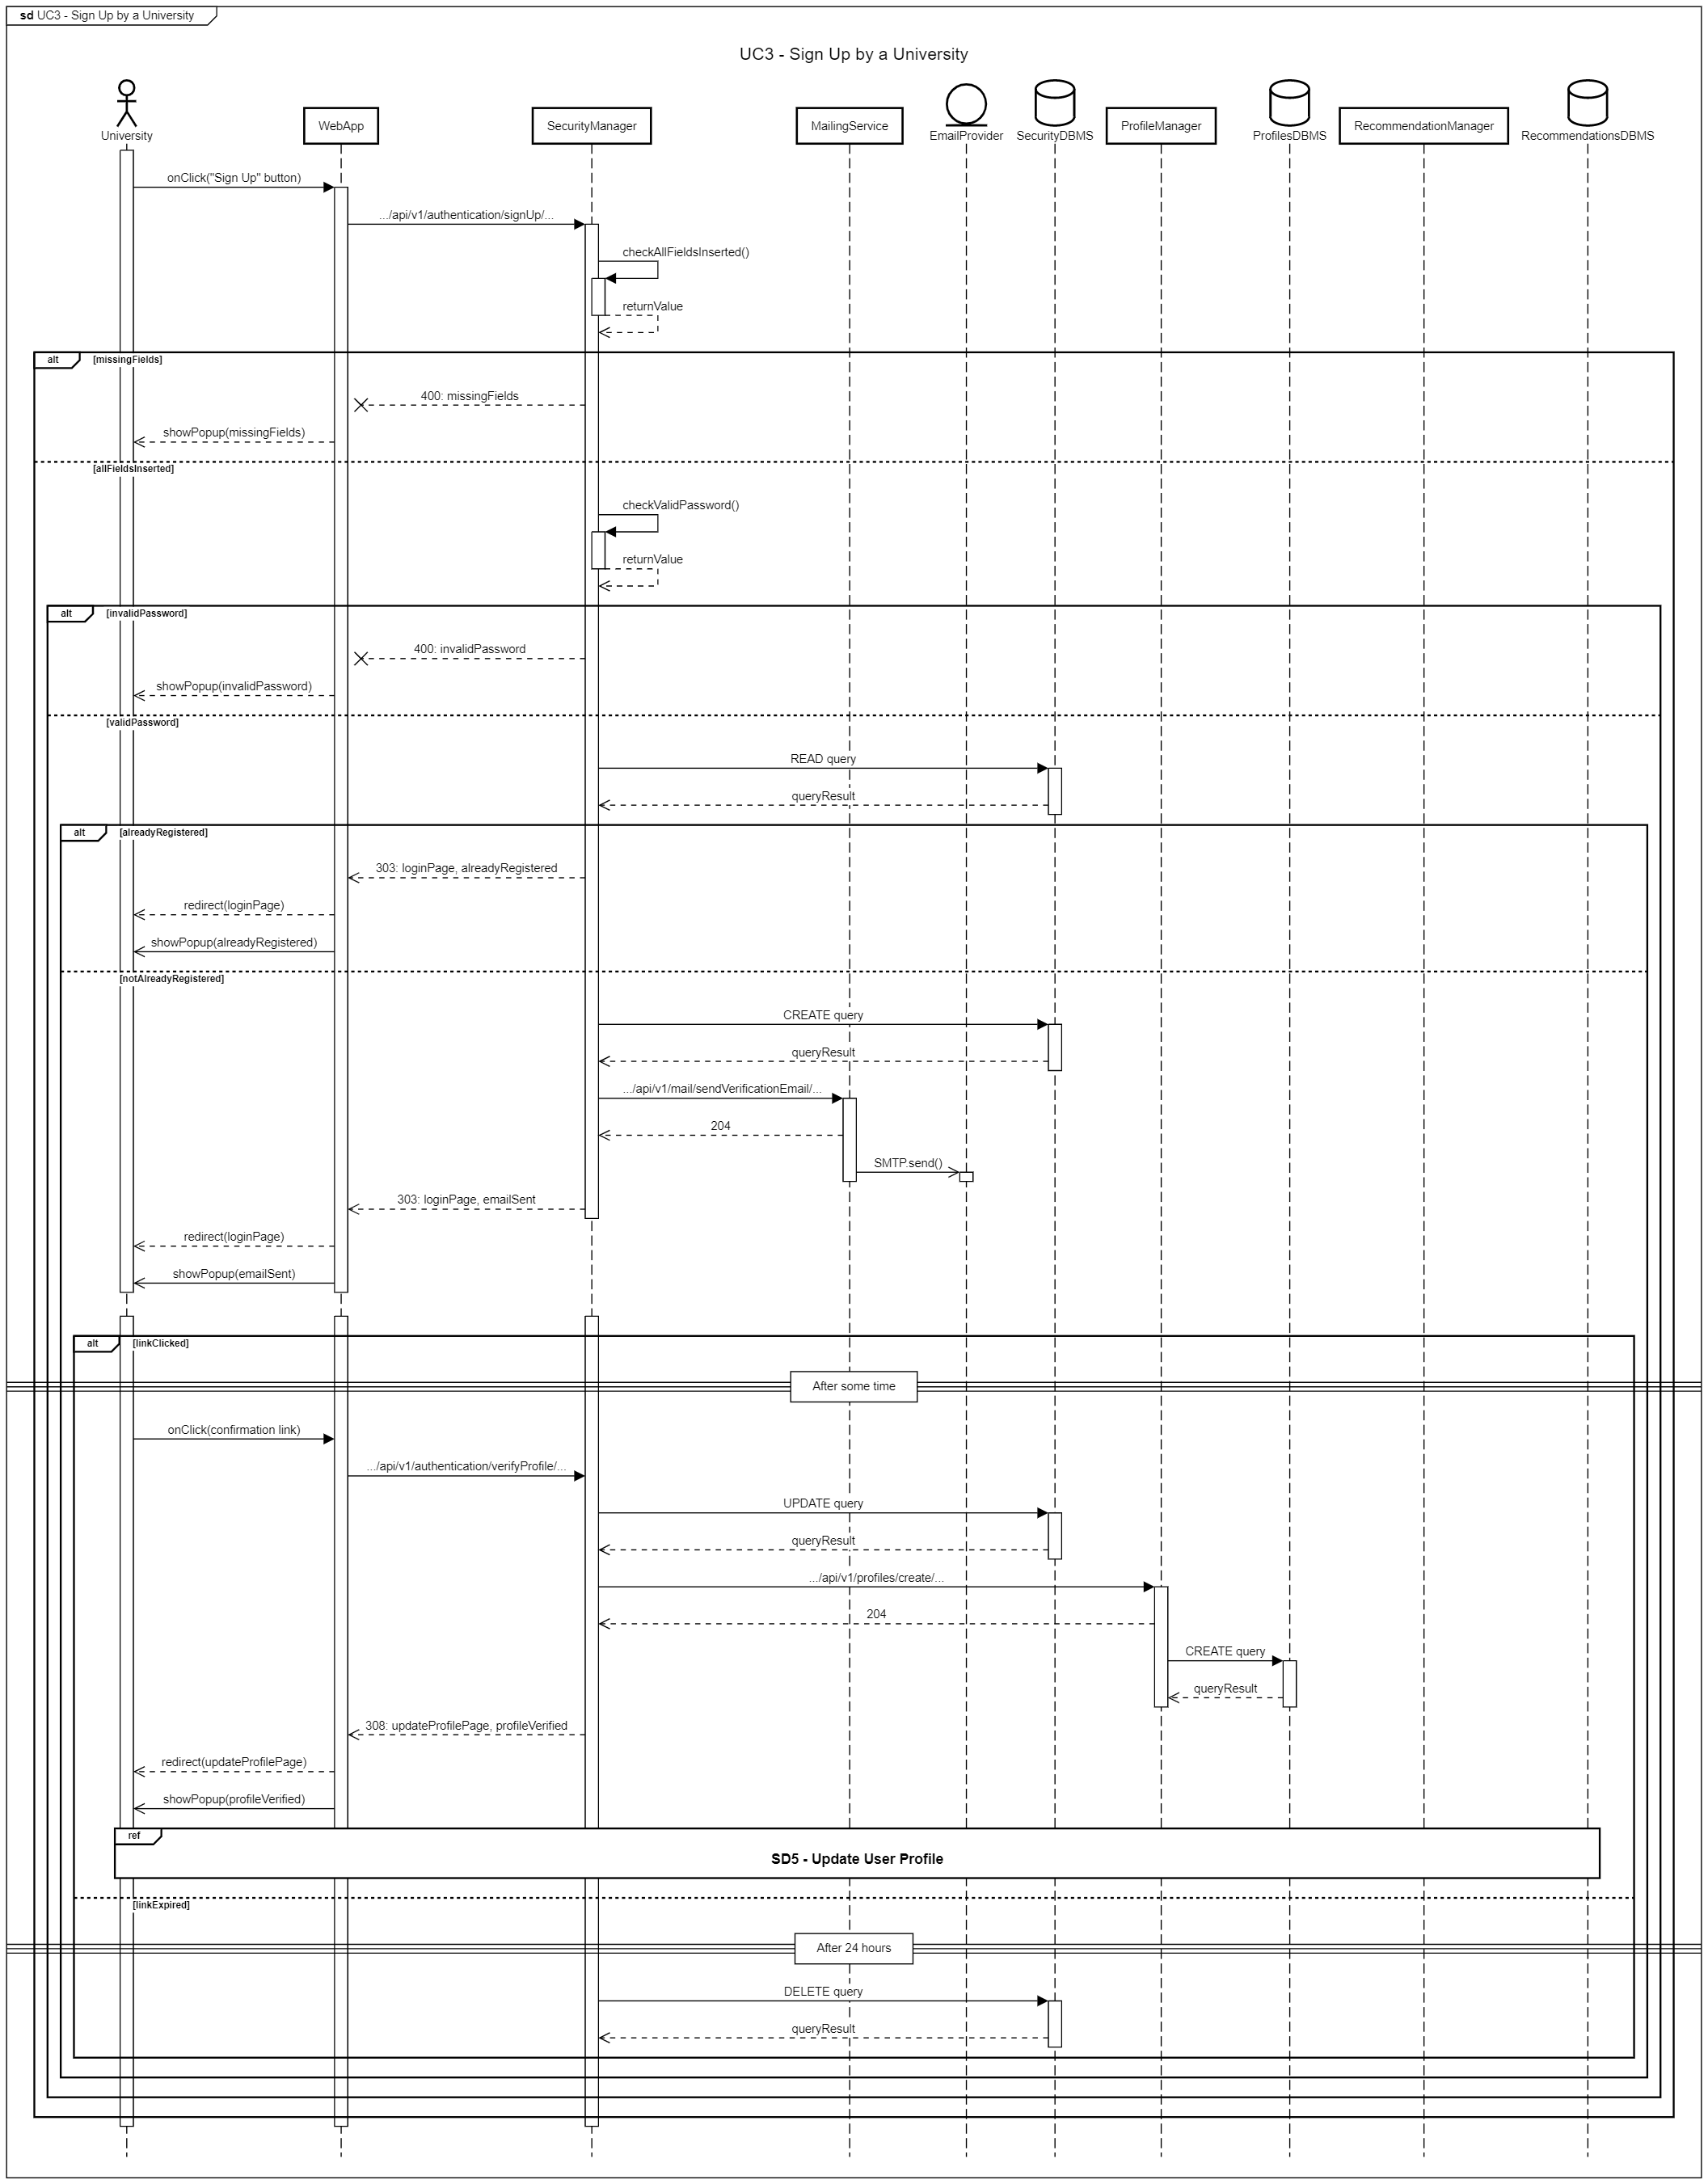
\includegraphics[width=0.9\linewidth]{LaTeXCode/images/SequenceDiagrams/UC3-sequenceDiagram.png}
         \caption{Sign Up by a University}
         \label{fig:signup_university_sd}
     \end{center}
\end{figure}

\subsubsection*{SD\cuc. Log In by a User}
\label{subsubsec:login_user_sd}
The User initiates the process by clicking the "Login" button on the login page, which sends a request to the \texttt{.../api/v1/authentication/login/...} API endpoint. The \texttt{SecurityManager} queries the \texttt{SecurityDBMS} to validate the provided credentials.
If the credentials are correct and the account is verified, the \texttt{SecurityManager} generates an authentication token, which is sent back to the \texttt{WebApp}. Then, the \texttt{SecurityManager} checks whether the User has completed their profile during the signup process. If the profile is incomplete, the User is sent the token and is redirected to the page for updating their profile in order for them to insert the required information; otherwise, they are redirected to the dashboard page with a success status and the token for authentication.

\begin{figure}[H]
    \begin{center}
         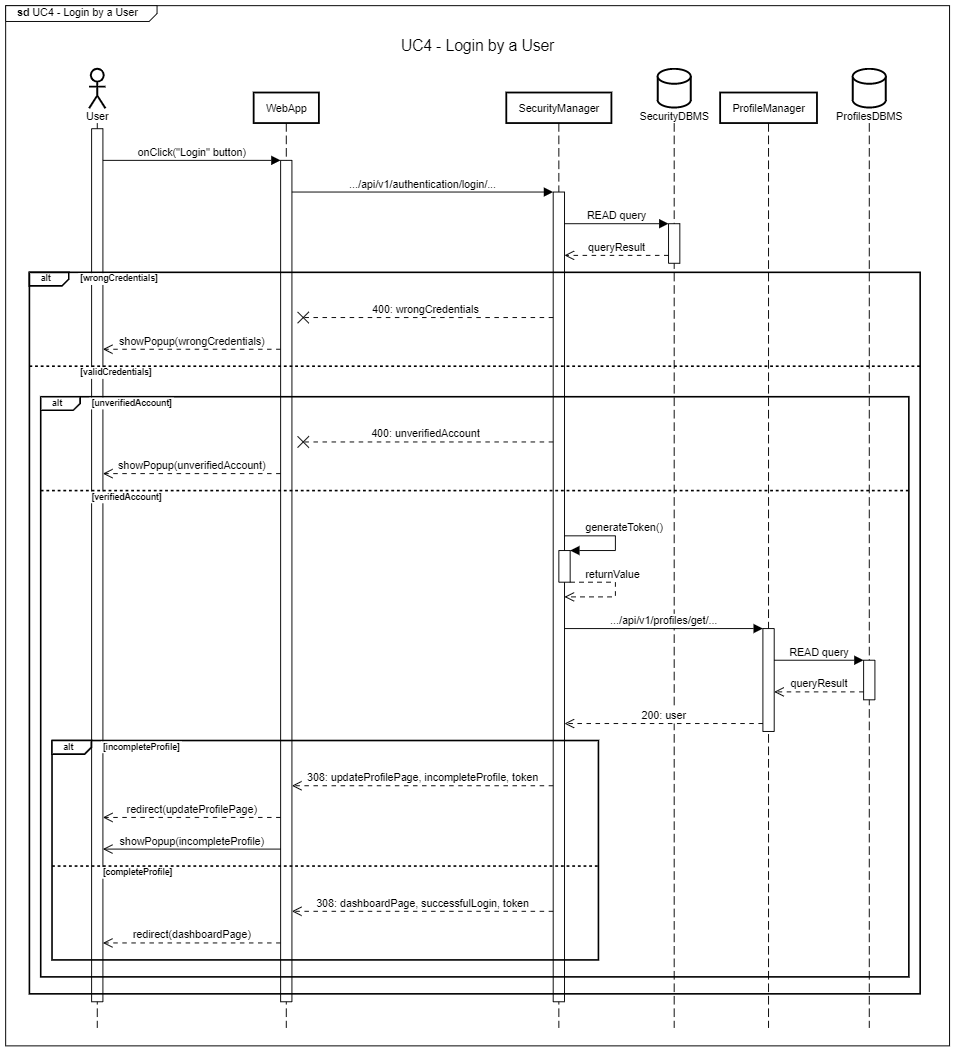
\includegraphics[width=0.8\linewidth]{LaTeXCode/images/SequenceDiagrams/UC4-sequenceDiagram.png}
         \caption{Log In by a User}
         \label{fig:login_user_sd}
     \end{center}
\end{figure}

\subsubsection*{SD\cuc. Update User Profile}
\label{subsubsec:update_profile_sd}
The User initiates the action by clicking the "Apply Changes" button after having inserted updated profile information in the profile update page, triggering a request to the \\ \texttt{.../api/v1/profiles/update/...} API endpoint. The \texttt{ProfileManager} validates the input to ensure all required fields are present.
If the input is valid, the \texttt{ProfileManager} updates the profile data in the \texttt{ProfilesDBMS}, and then notifies the successful update to the WebApp, which shows a popup to the User. The \texttt{ProfileManager} then triggers the \texttt{RecommendationManager} to execute the logic of \hyperref[fig:generate_recommendations_sd]{\protect\uline{SD10 - Generate Recommendations}} for detecting possible new recommendations to be generated.

\begin{figure}[H]
    \begin{center}
         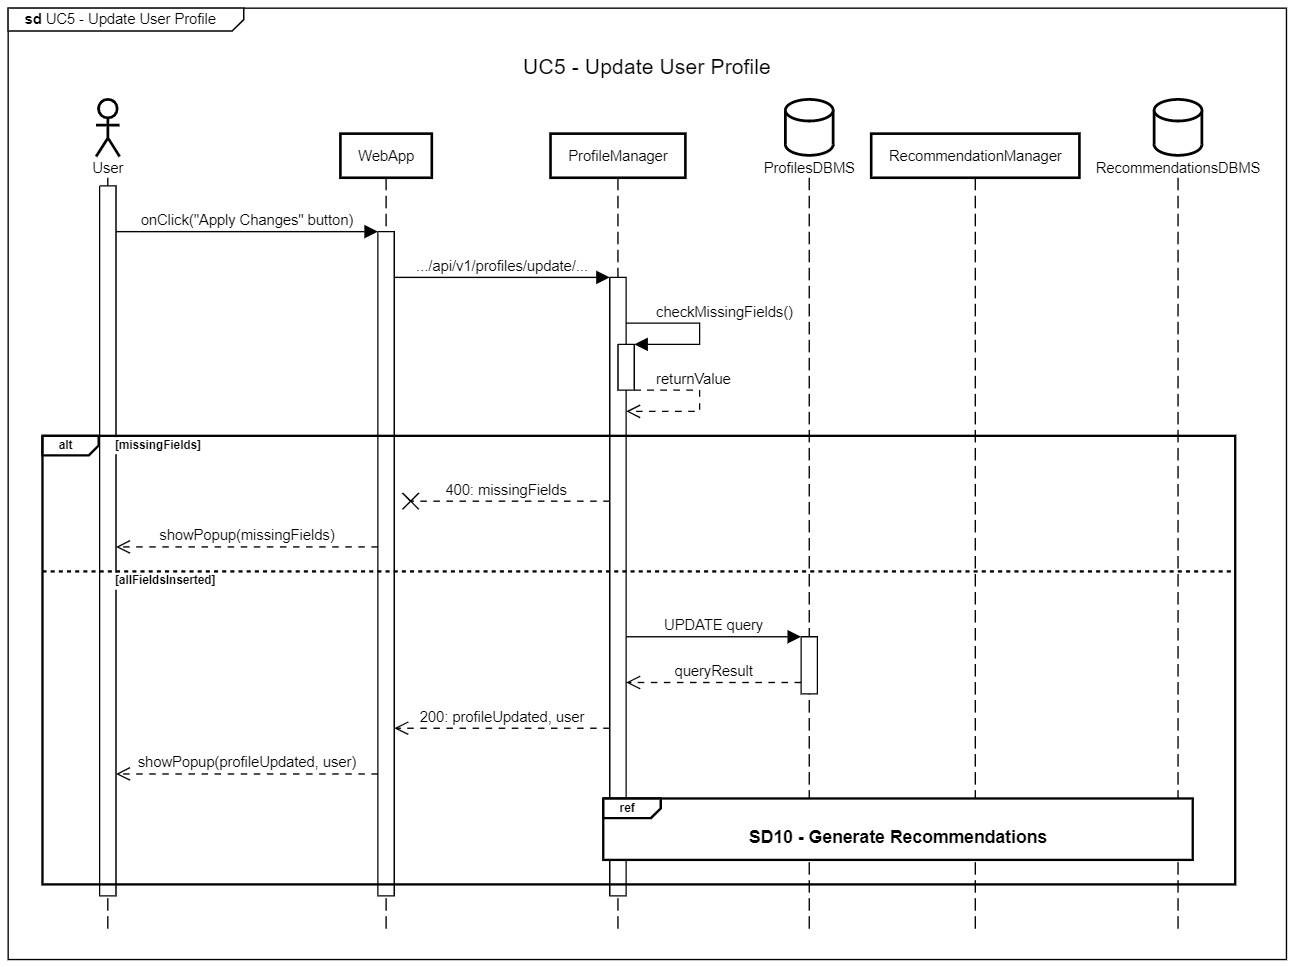
\includegraphics[width=1\linewidth]{LaTeXCode/images/SequenceDiagrams/UC5-sequenceDiagram.png}
         \caption{Update User Profile}
         \label{fig:update_profile_sd}
     \end{center}
\end{figure}

\newpage

\subsubsection*{SD\cuc. Publish an Internship Offer}
\label{subsubsec:publish_offer_sd}
The Company initiates the action by clicking the "Submit" button after having inserted information about the new offer to be posted in the offer creation page, which sends a request to the \texttt{.../api/v1/offers/publish/...} API endpoint. The \texttt{OfferManager} validates the input to ensure all required fields are completed.
If all fields are provided and all the information is compliant the \texttt{OfferManager} creates a new entry in the \texttt{InternshipsDBMS}.
Once the query succeeds, the \texttt{OfferManager} confirms the offer's publication and the Company is notified with a popup indicating that the offer has been successfully published. The component then triggers the \texttt{RecommendationManager} to generate recommendations as part of \hyperref[fig:generate_recommendations_sd]{\protect\uline{SD10 - Generate Recommendations}}.

\begin{figure}[H]
    \begin{center}
         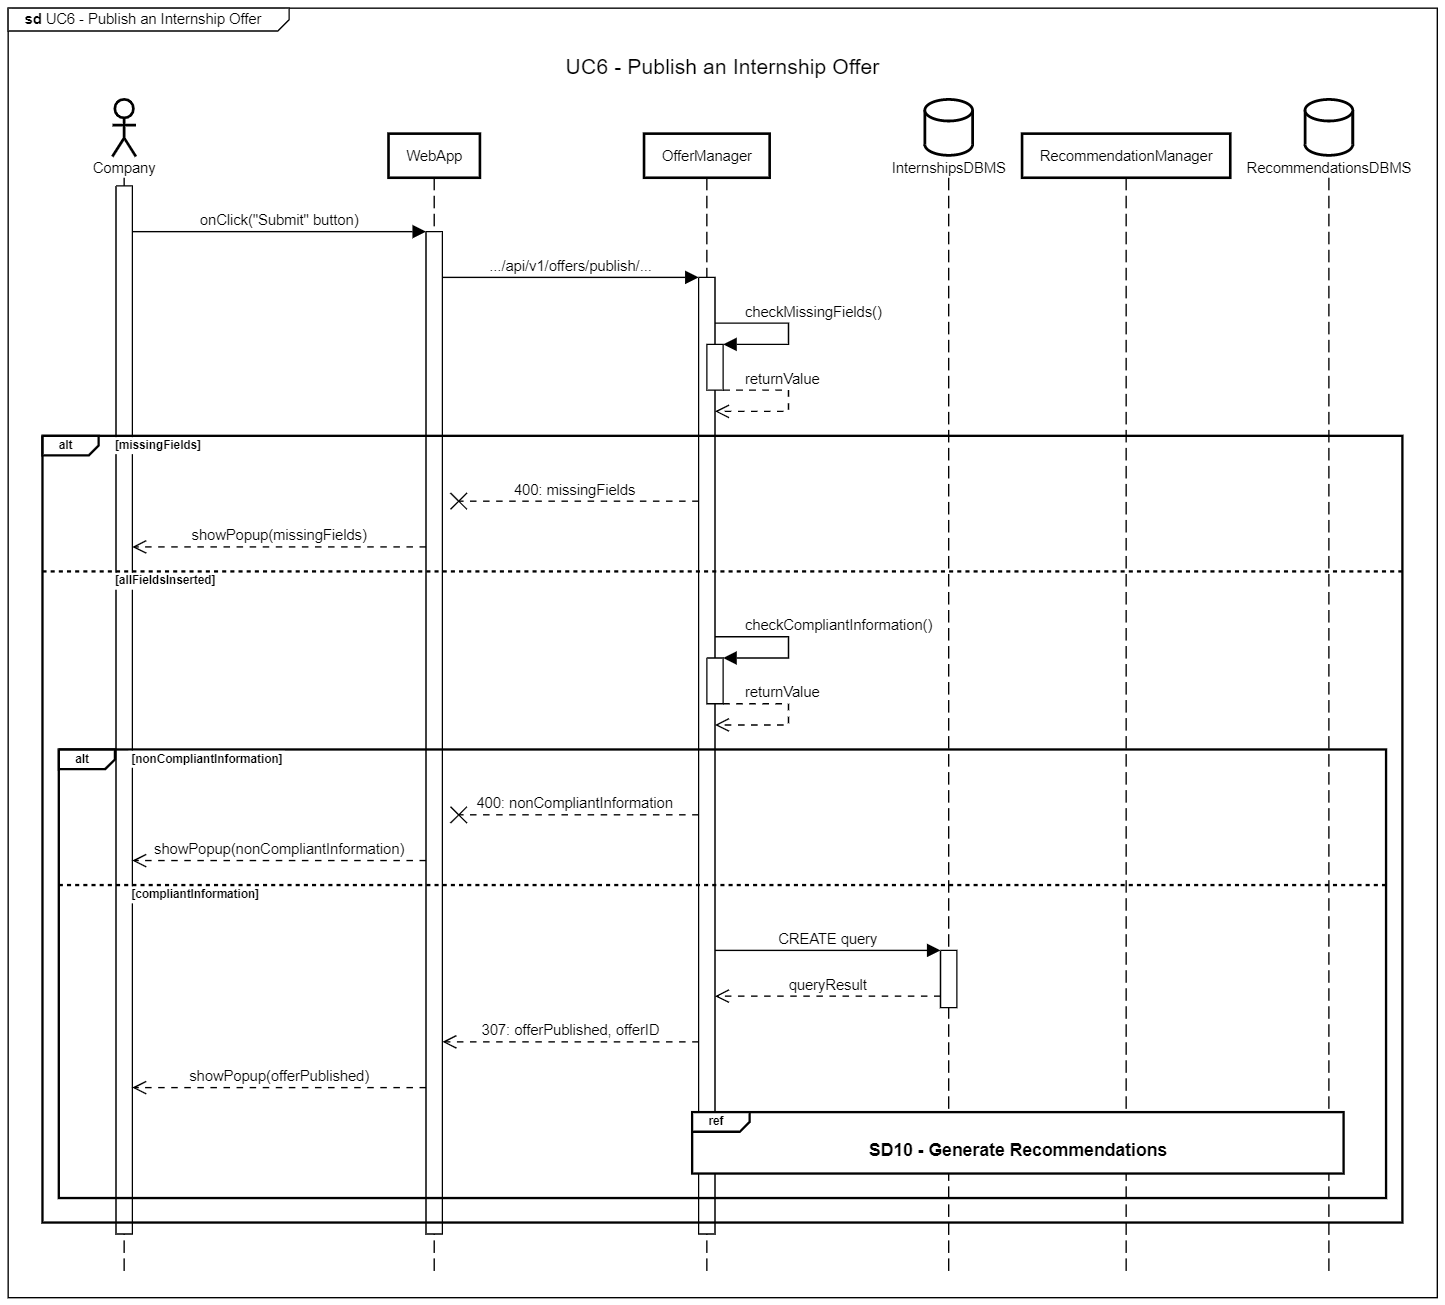
\includegraphics[width=1\linewidth]{LaTeXCode/images/SequenceDiagrams/UC6-sequenceDiagram.png}
         \caption{Publish an Internship Offer}
         \label{fig:publish_offer_sd}
     \end{center}
\end{figure}

\subsubsection*{SD\cuc. Update Internship Offer}
\label{subsubsec:update_internship_offer_sd}
The Company initiates the action either by confirming the withdrawal or by applying changes to one of its offers on the page dedicated to that specific offer. For the withdrawal, the \\ \texttt{.../api/v1/offers/withdraw/...} API endpoint is the one where the request is sent. The \texttt{OfferManager} retrieves related "Unhandled" recommendations by interacting with the \\ \texttt{RecommendationManager}, which in turn queries the \texttt{RecommendationsDBMS}, and subsequently asks the exposed API to discard them. Then the \texttt{OfferManager} doesn't DELETE the offer, but only performs an UPDATE query for its status in the \texttt{InternshipsDBMS}, so that its data doesn't get lost. Finally, the component redirects the Company to the dashboard with a success alert.
When updating offer information, the request is instead forwarded to the \texttt{.../api/v1/offers/update/...} API endpoint. The \texttt{OfferManager} validates the input for missing fields and compliance. If valid, the updated information is stored in the \texttt{InternshipsDBMS}, and the system notifies the Company of the successful update, in the end triggering the \texttt{RecommendationManager} to generate new recommendations as defined in \hyperref[fig:generate_recommendations_sd]{\protect\uline{SD10 - Generate Recommendations}}.

\newpage

\begin{figure}[H]
    \begin{center}
         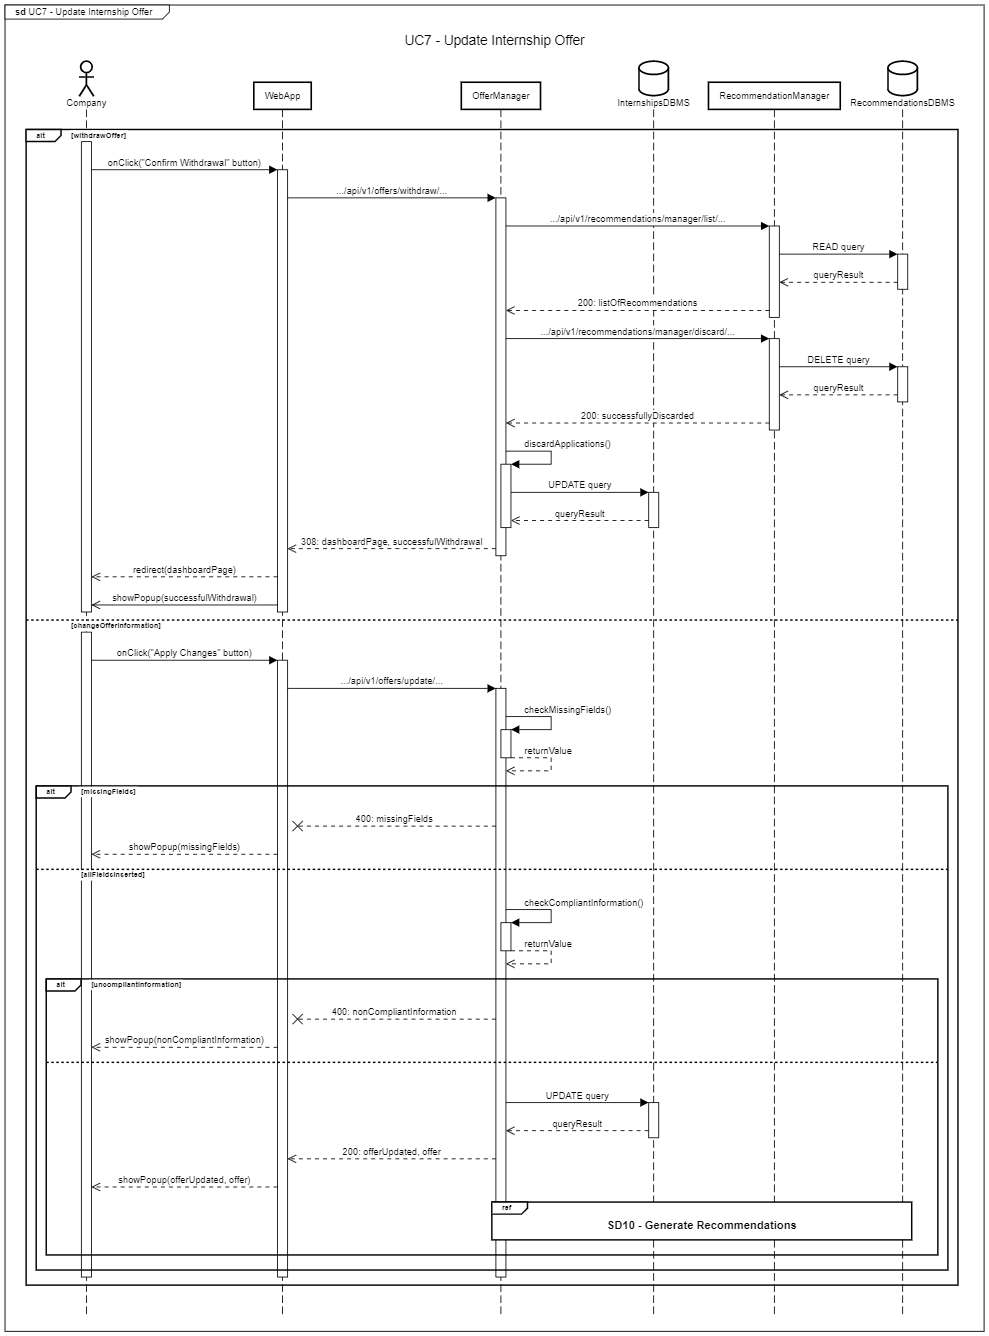
\includegraphics[width=1\linewidth]{LaTeXCode/images/SequenceDiagrams/UC7-sequenceDiagram.png}
         \caption{Update Internship Offer}
         \label{fig:update_internship_offer_sd}
     \end{center}
\end{figure}

\subsubsection*{SD\cuc. Search Internship Offers}
\label{subsubsec:search_offer_sd}
The Student initiates the action by clicking the "Submit" button on the dashboard page after having inserted the filter criteria, triggering a request to the \texttt{.../api/v1/offers/search/...} API endpoint. The \texttt{OfferManager} processes the request and queries the \texttt{InternshipsDBMS} using a READ operation to fetch the relevant internship offers which match the search query criteria.
The \texttt{OfferManager} returns the query results to the \texttt{WebApp}, which displays the results to the Student. If no results are found, the system shows a custom message of the list of internships instead.

\begin{figure}[H]
    \begin{center}
         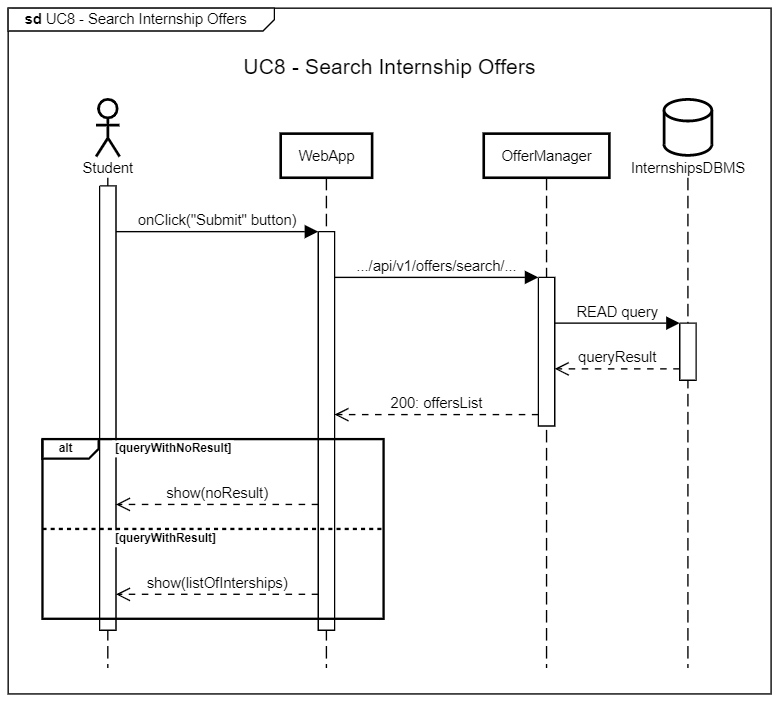
\includegraphics[width=1\linewidth]{LaTeXCode/images/SequenceDiagrams/UC8-sequenceDiagram.png}
         \caption{Search Internship Offers}
         \label{fig:search_offer_sd}
     \end{center}
\end{figure}

\subsubsection*{SD\cuc. Apply to an Internship Offer}
\label{subsubsec:apply_to_internships_sd}
The Student submits an application for an internship offer by clicking the "Apply" button on an offer's page, invoking the \texttt{.../api/v1/offers/apply/...} API endpoint. The \texttt{OfferManager} first verifies the deadline through the \texttt{InternshipsDBMS}: if the deadline has expired, an error is shown to the Student; otherwise, the \texttt{OfferManager} calls the \texttt{RecommendationManager}, which interacts with the \texttt{RecommendationsDBMS} to accept the recommendations of the applicating Student about that offer and to discard the recommendations of the offering Company about that Student for that Offer, as expected by the functional requirements. Finally, the application is recorded in the \texttt{InternshipsDBMS}, and the Student is notified of the successful submission.

\begin{figure}[H]
    \begin{center}
         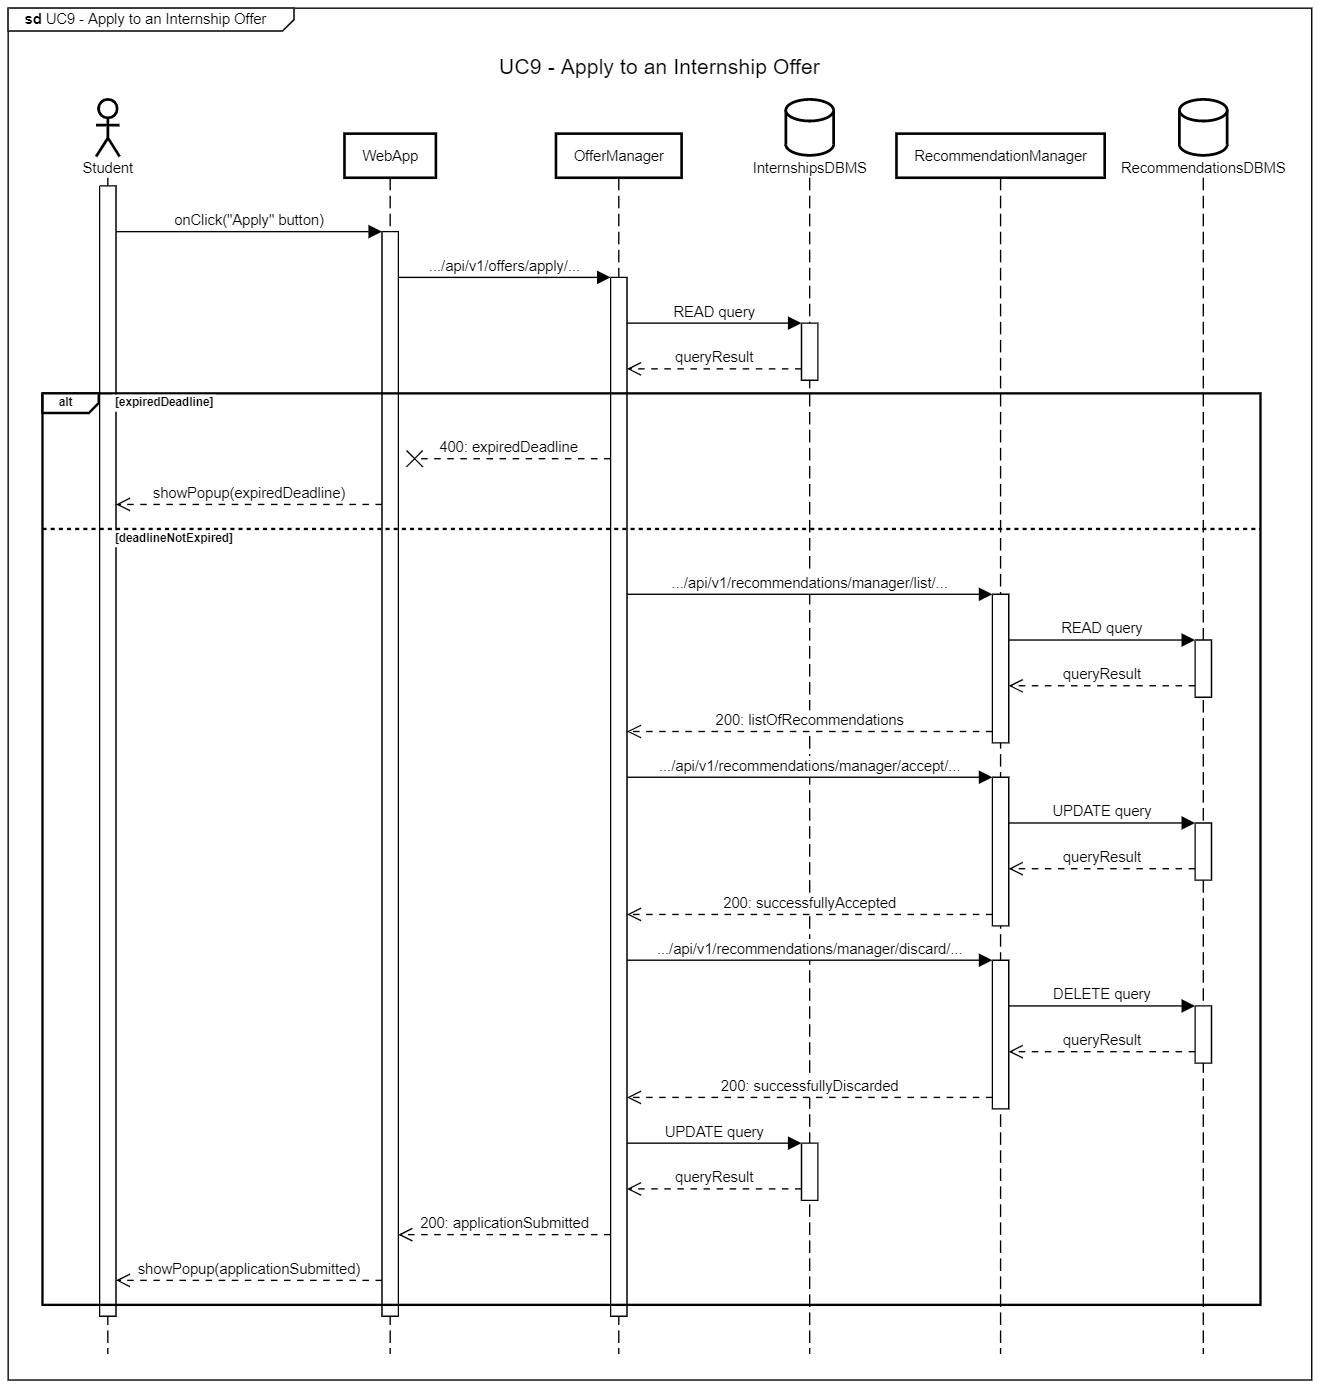
\includegraphics[width=0.9\linewidth]{LaTeXCode/images/SequenceDiagrams/UC9-sequenceDiagram.png}
         \caption{Apply to an Internship Offer}
         \label{fig:apply_to_internships_sd}
     \end{center}
\end{figure}

\subsubsection*{SD\cuc. Generate Recommendations}
\label{subsubsec:generate_recommendations_sd}
The process can be triggered either by a profile update through the \texttt{ProfileManager} or an internship offer update via the \texttt{OfferManager}, both invoking the \\ \texttt{.../api/v1/recommendations/generator/generate/...} API endpoint.
Upon invocation, the \texttt{RecommendationManager} queries the \texttt{RecommendationDBMS} to retrieve relevant data for generating new recommendations. Once the query is completed and the data is processed, the new recommendations are pushed into the \texttt{RecommendationDBMS}.

\begin{figure}[H]
    \begin{center}
         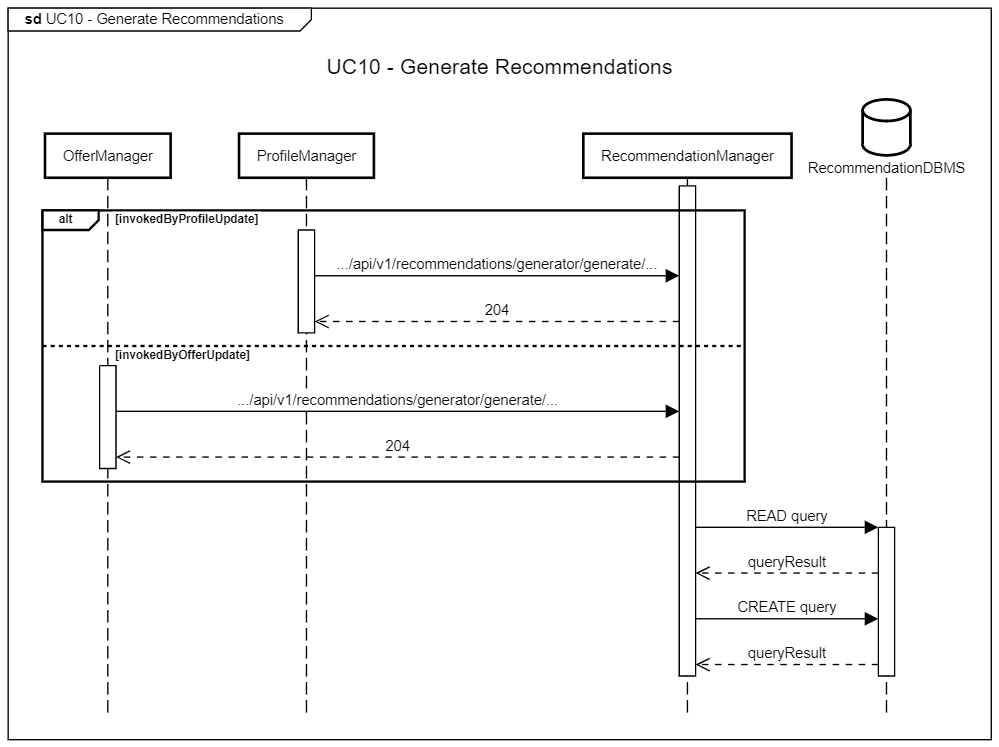
\includegraphics[width=1\linewidth]{LaTeXCode/images/SequenceDiagrams/UC10-sequenceDiagram.png}
         \caption{Generate Recommendations}
         \label{fig:generate_recommendations_sd}
     \end{center}
\end{figure}

\newpage

\subsubsection*{SD\cuc. Manage Internship Recommendations}
\label{subsubsec:manage_internship_recommendations_sd}
For each of their "Unhandled" recommendations, the Student can either accept it, reject it, or postpone the decision. Whether the Student clicks the "Accept" or the "Reject" button on a recommendation's widget, triggering the corresponding \texttt{.../api/v1/recommendations/manager/...} API endpoint of the \texttt{RecommendationManager}, the status of the recommendation in the \\ \texttt{RecommendationsDBMS} is updated accordingly. In case of acceptance, an application for the offer from the Student is also generated, as discussed in the functional requirements, by invoking \hyperref[fig:apply_to_internships_sd]{\protect\uline{SD9 - Apply to an Internship Offer}}. A confirmation popup for the success of the operation is finally displayed to the Student. Recommendations postponed (for which no action is taken) remain unaltered.

\begin{figure}[H]
    \begin{center}
         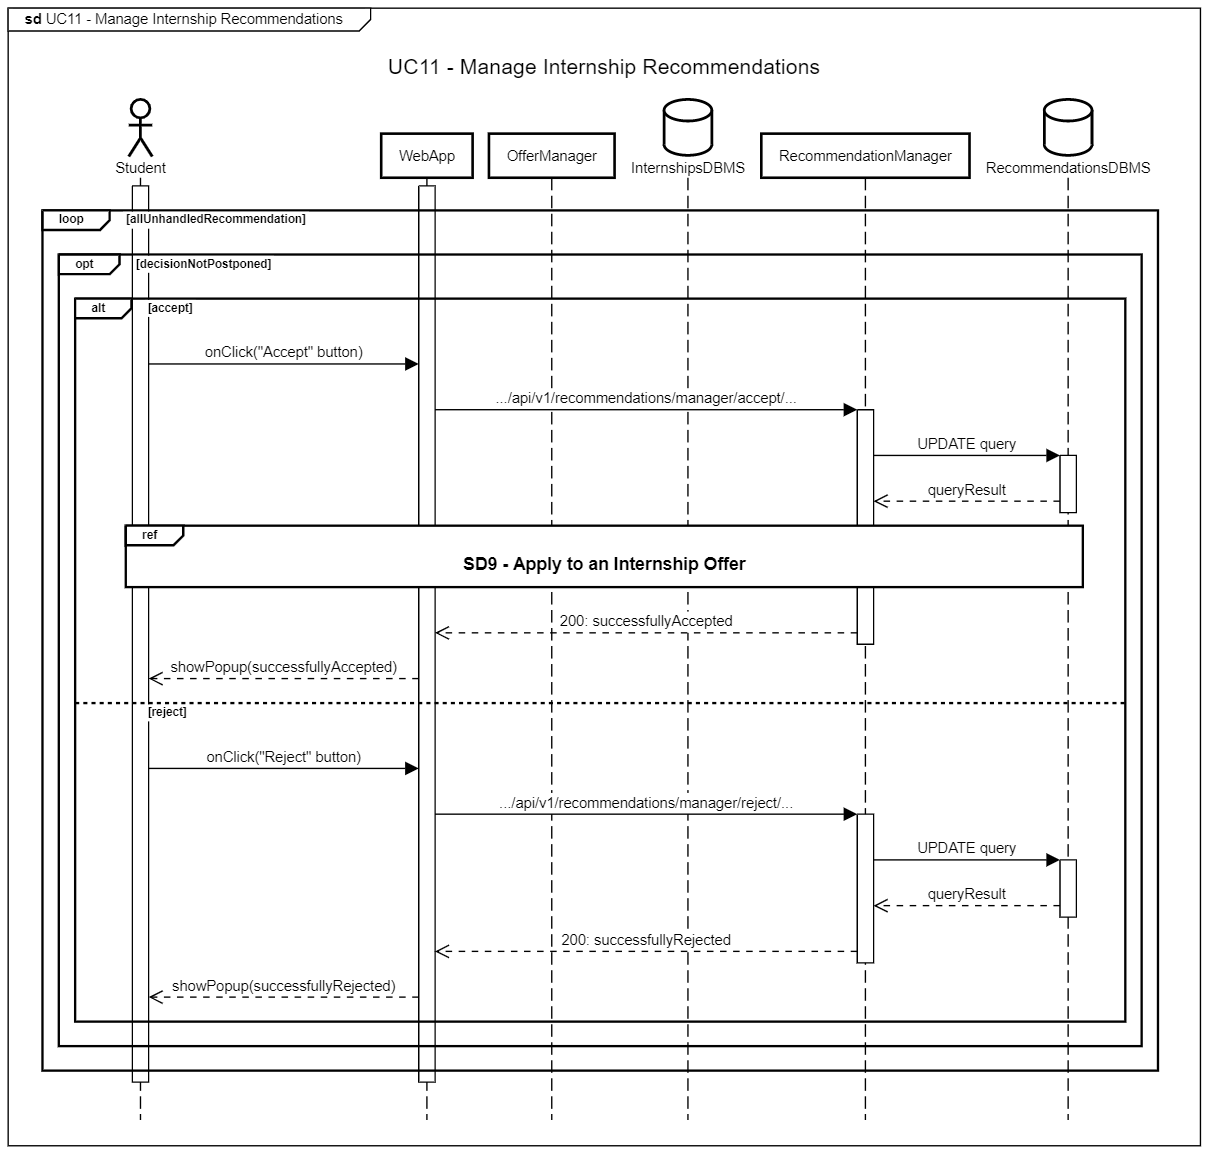
\includegraphics[width=0.9\linewidth]{LaTeXCode/images/SequenceDiagrams/UC11-sequenceDiagram.png}
         \caption{Manage Internship Recommendations}
         \label{fig:manage_internship_recommendations_sd}
     \end{center}
\end{figure}

\subsubsection*{SD\cuc. Manage Students Recommendations}
\label{subsubsec:manage_students_recommendations_sd}
Similar to the previous one, the following Sequence Diagram describes the process of recommendations management by a Company. The only difference is that, instead of generating an offer application, when accepting a recommendation a new one is generated for the corresponding Student if they don't already have one.

\begin{figure}[H]
    \begin{center}
         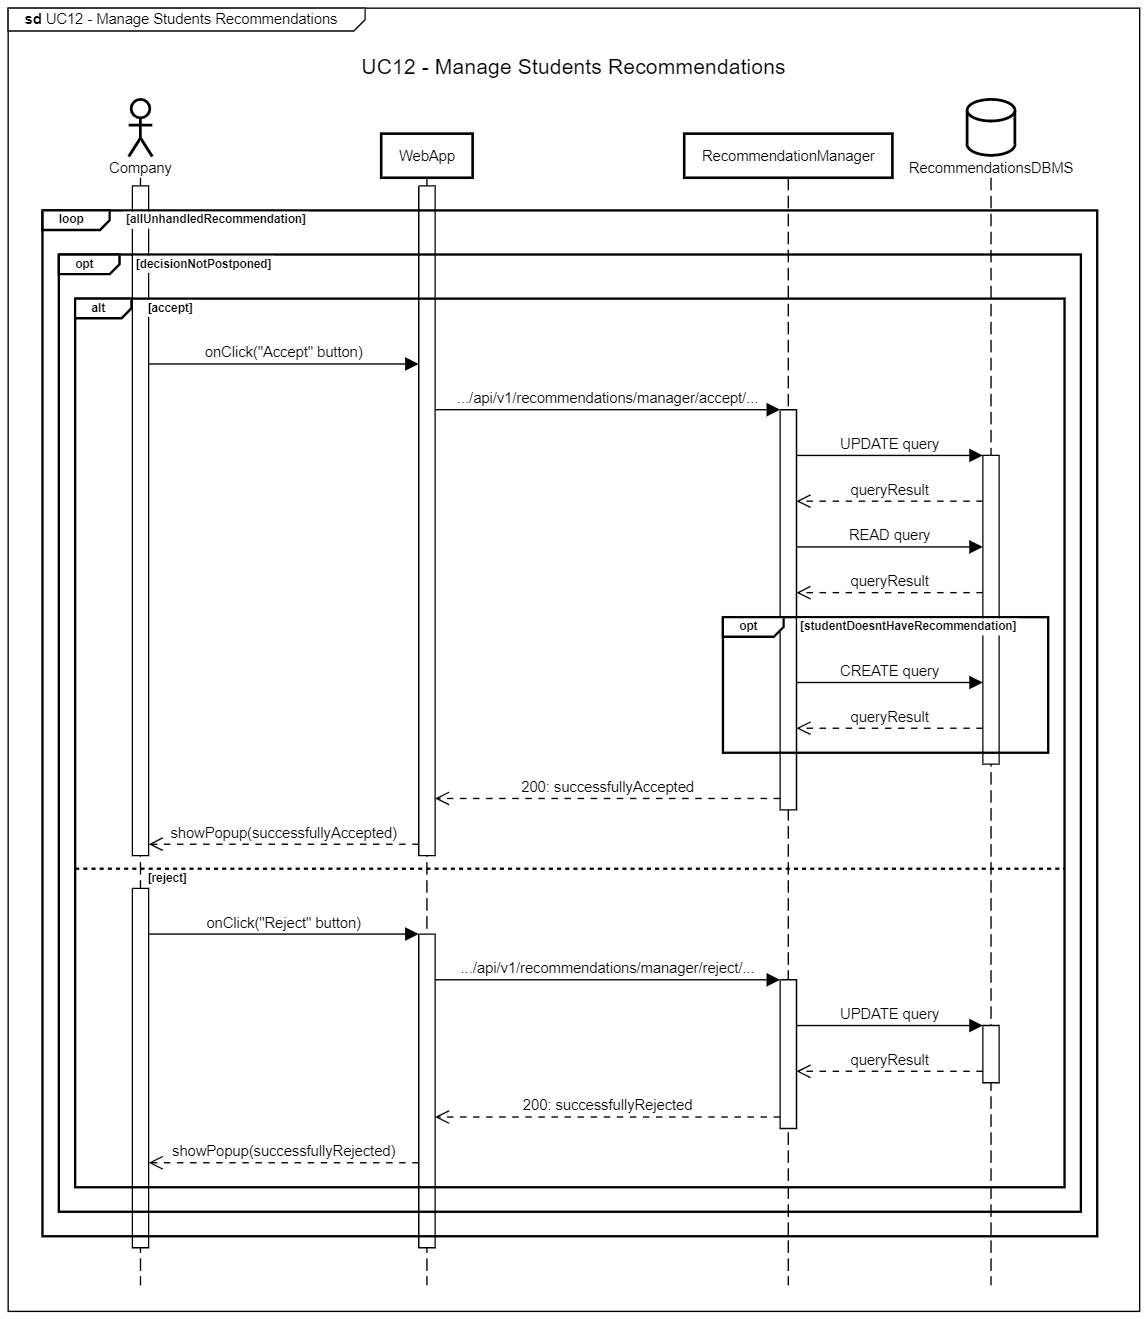
\includegraphics[width=0.9\linewidth]{LaTeXCode/images/SequenceDiagrams/UC12-sequenceDiagram.png}
         \caption{Manage Students Recommendations}
         \label{fig:manage_students_recommendations_sd}
     \end{center}
\end{figure}

\subsubsection*{SD\cuc. Manage an Interview}
\label{subsubsec:manage_interview_sd}
This Sequence Diagram illustrates the process of scheduling, conducting, and evaluating an interview between a Company and a Student.
\begin{enumerate}
    \item The Company first clicks the "Send Invitation" button on its dashboard, sending an interview invitation through the \texttt{.../api/v1/interviews/sendInvitation/...} API endpoint, managed by the \texttt{InterviewManager}, which creates an entry in the \texttt{InternshipsDBMS} for the invitation. The Student may accept or decline the invitation by clicking the corresponding buttons, which invoke the respective \texttt{.../api/v1/internships/...} API endpoint:
    \begin{itemize}
        \item If accepted, the \texttt{InterviewManager} updates the status in the \texttt{InternshipsDBMS}, and the Student is notified.
        \item If declined, the \texttt{InternshipsDBMS} is updated accordingly, and the Company may decide to try to reschedule it based on the motivation provided by the Student.
    \end{itemize}
    This phase loops until either the Student accepts one invitation, or the Company decides that no agreement can be reached and stops the process.
    
    \item For in-platform interviews only, the Company posts some questions via the "Post Questions" button, which calls the \texttt{.../api/v1/interviews/createQuestions/...} API endpoint, and when the scheduled time comes the Student involved in the interview replies to each question and submits their answer through the "Submit" button of the specific question in its dashboard, which interacts with the system through the \\ \texttt{.../api/v1/interviews/submitAnswer/...} API endpoint. The questions and the answers are recorded in the \texttt{InternshipsDBMS}, and popups are shown to both parties to confirm their submissions.

    \item After the interview, the Company evaluates the candidate by submitting the results through the specific "Evaluate" button, calling \texttt{.../api/v1/interviews/evaluate/...} API endpoint. The result and eventual feedback are stored in the \texttt{InternshipsDBMS} by updating the interview status, and the Company is notified of the successful evaluation.
\end{enumerate}

\newpage

\begin{figure}[H]
    \begin{center}
         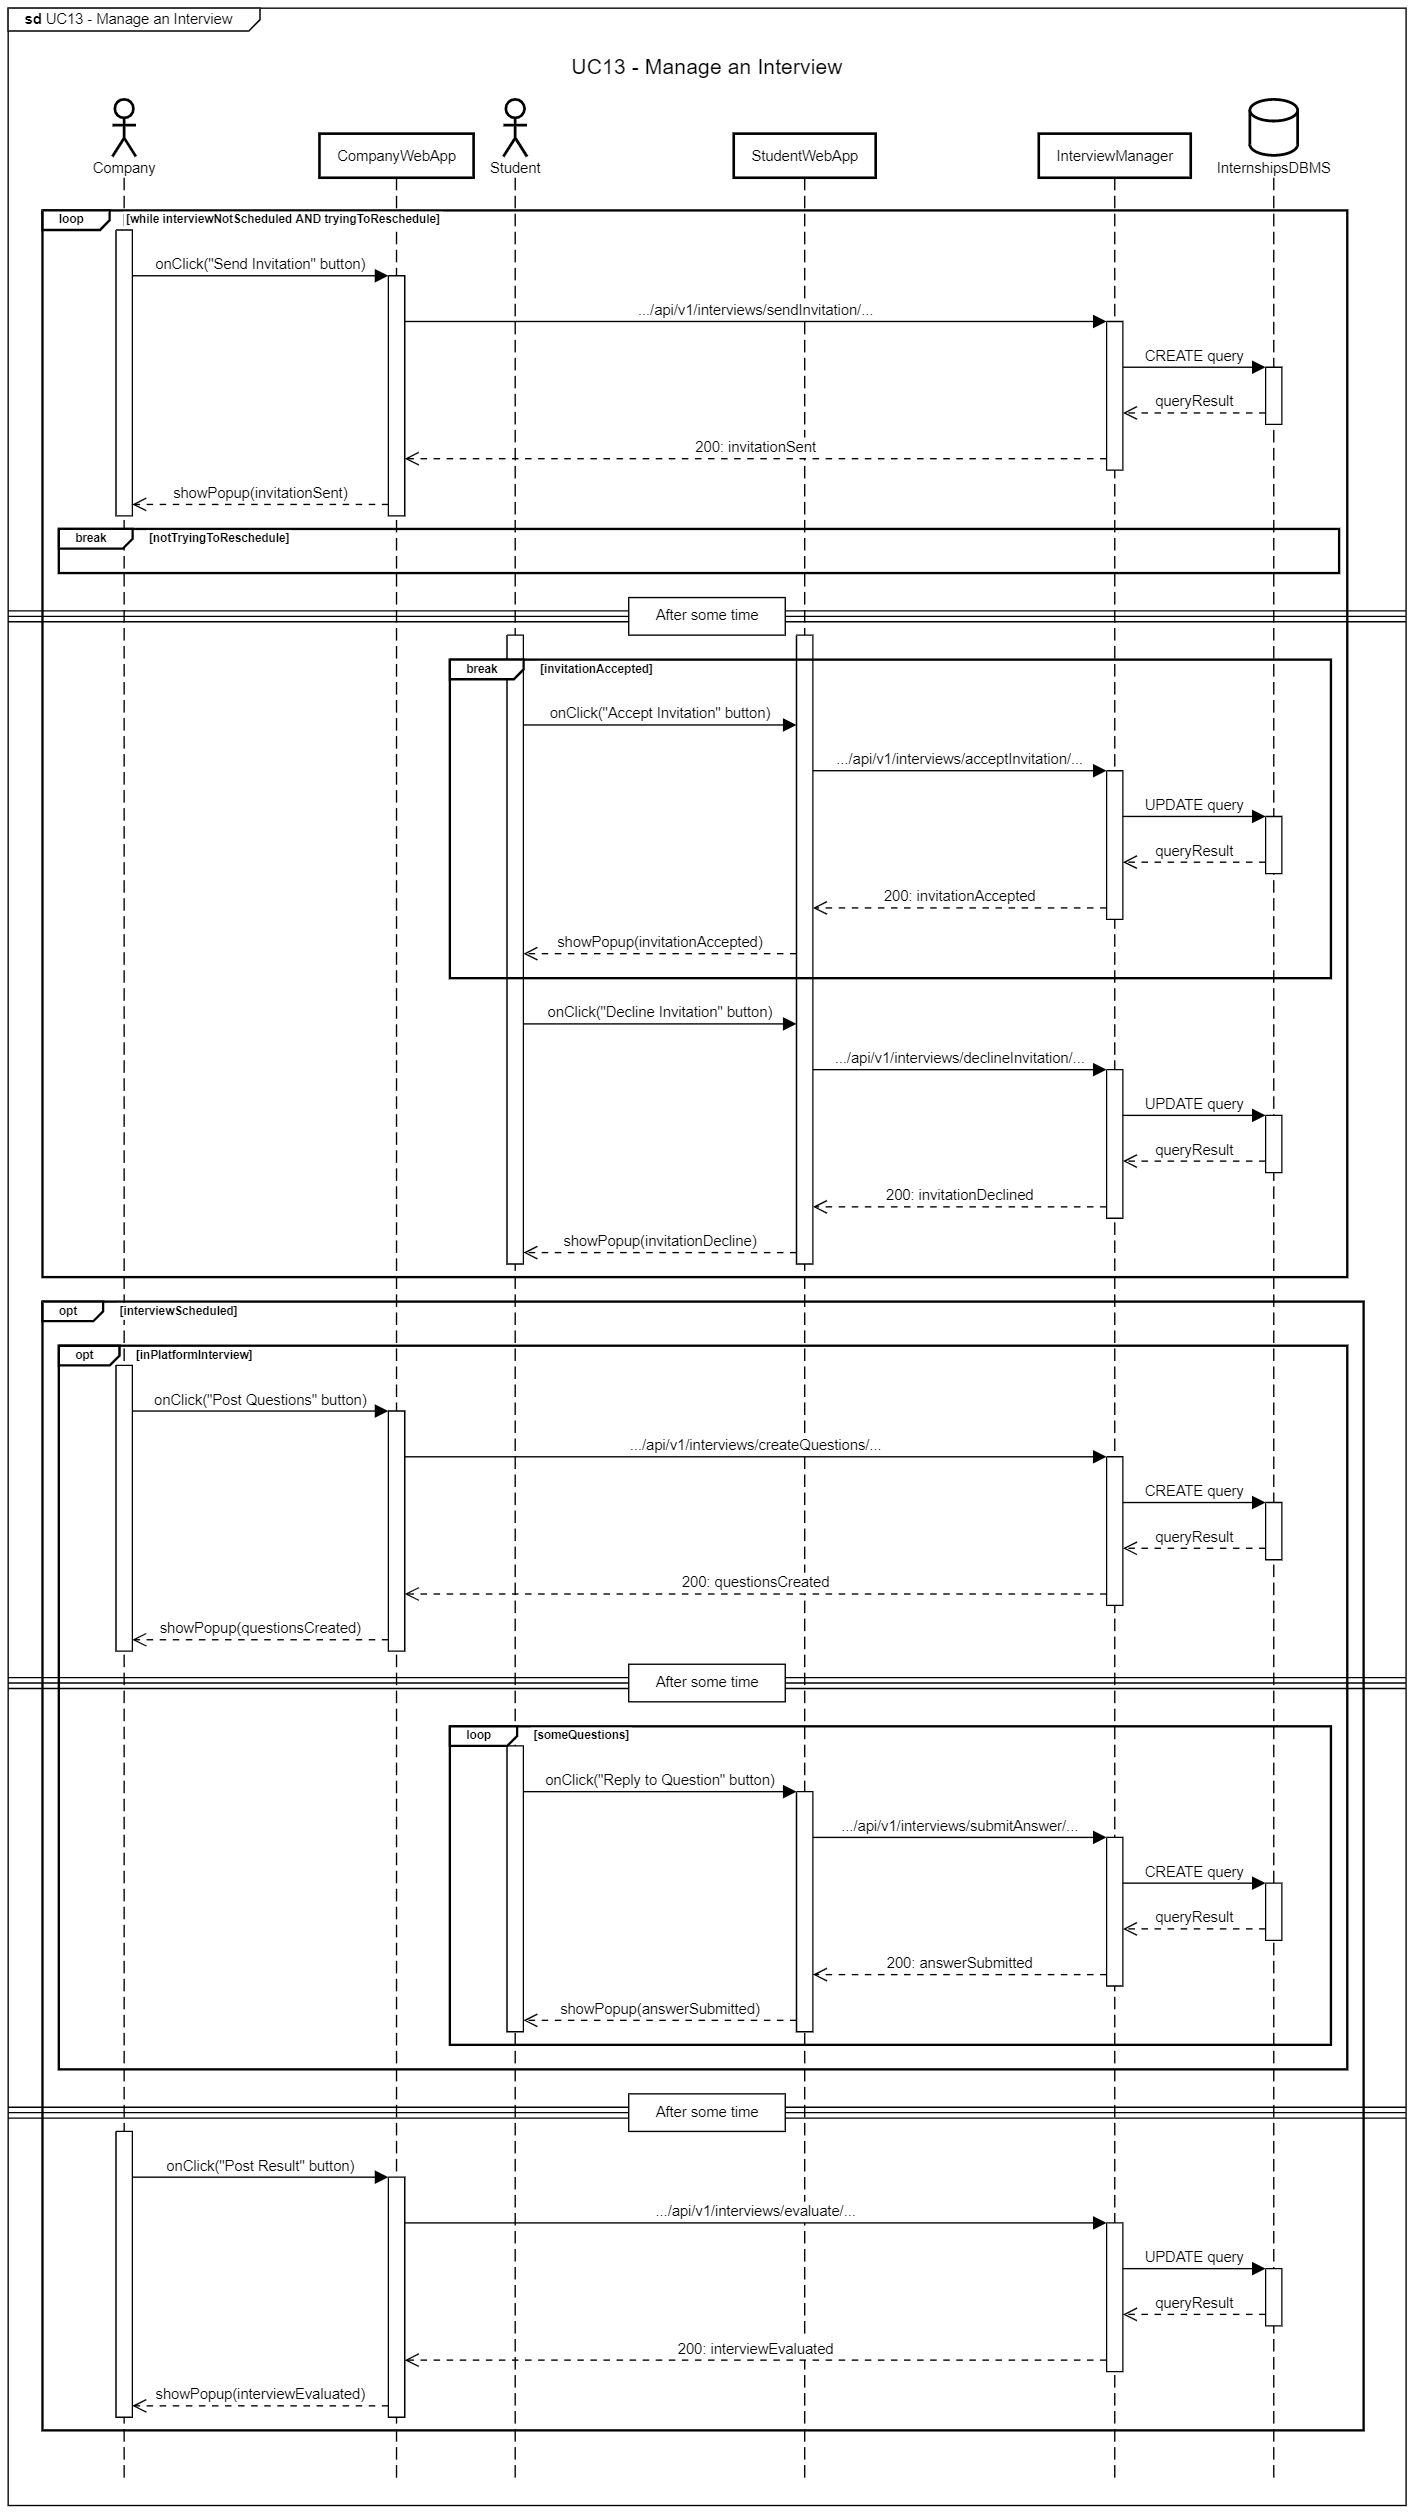
\includegraphics[width=0.8\linewidth]{LaTeXCode/images/SequenceDiagrams/UC13-sequenceDiagram.png}
         \caption{Manage an Interview}
         \label{fig:manage_interview_sd}
     \end{center}
\end{figure}

\subsubsection*{SD\cuc. Provide Information for an ongoing Internship}
\label{subsubsec:provide_information_ongoing_sd}
The Party initiates the process by clicking the "Post Information"  on an ongoing internship's page, which triggers a request to the \texttt{.../api/v1/internships/addInformation/...} API endpoint handled by the \texttt{IMFManager}. The \texttt{IMFManager} adds the new internship data in the \texttt{InternshipsDBMS}. Once the operation is successfully completed, the \texttt{WebApp} receives a confirmation and displays a popup notifying the Party of the successful submission.

\begin{figure}[H]
    \begin{center}
         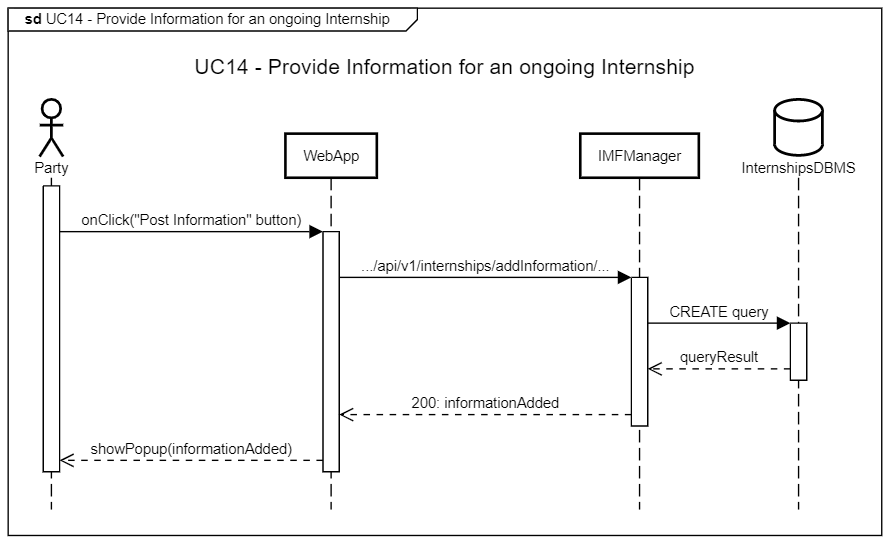
\includegraphics[width=1\linewidth]{LaTeXCode/images/SequenceDiagrams/UC14-sequenceDiagram.png}
         \caption{Provide Information for an ongoing Internship}
         \label{fig:provide_information_ongoing_sd}
     \end{center}
\end{figure}

\newpage

\subsubsection*{SD\cuc. Monitor an ongoing Internship}
\label{subsubsec:monitor_internship_sd}
The Party selects an internship widget, sending a request to the \texttt{.../api/v1/internships/get/...} API endpoint handled by the \texttt{IMFManager}. The \texttt{IMFManager} retrieves the internship details from the \texttt{InternshipsDBMS}. Upon successfully fetching the data, the \texttt{WebApp} displays the internship details to the Party.
Additionally, in the visualized section the Party can also optionally provide new information about the internship if they need to, referring to the process detailed in \hyperref[fig:provide_information_ongoing_sd]{\protect\uline{SD14 - Provide Information for an ongoing Internship}}.

\begin{figure}[H]
    \begin{center}
         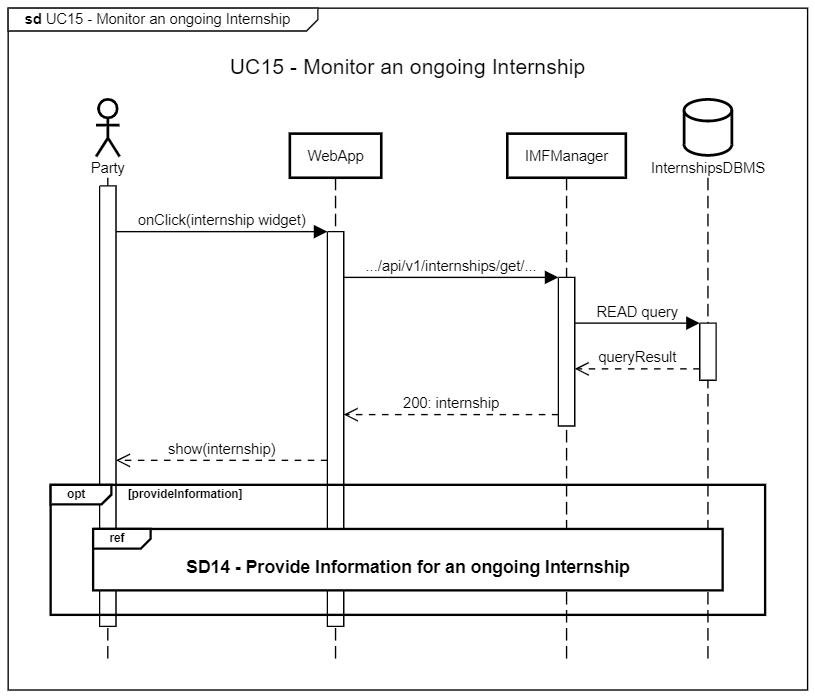
\includegraphics[width=1\linewidth]{LaTeXCode/images/SequenceDiagrams/UC15-sequenceDiagram.png}
         \caption{Monitor an ongoing Internship}
         \label{fig:monitor_internship_sd}
     \end{center}
\end{figure}

\newpage

\subsubsection*{SD\cuc. Report Problems during an Internship}
\label{subsubsec:report_problems_sd}
The Party initiates the process by clicking the "Report" button on an ongoing internship's page, triggering a request to the \texttt{.../api/v1/internships/reportProblem/...} API endpoint exposed by the \texttt{IMFManager}, which checks the submitted fields for completeness. If all fields are provided, the \texttt{IMFManager} records the problem in the \texttt{InternshipsDBMS} creating a new entry. Once the problem is successfully reported, the \texttt{WebApp} notifies the Party with the appropriate confirmation popup.

\begin{figure}[H]
    \begin{center}
         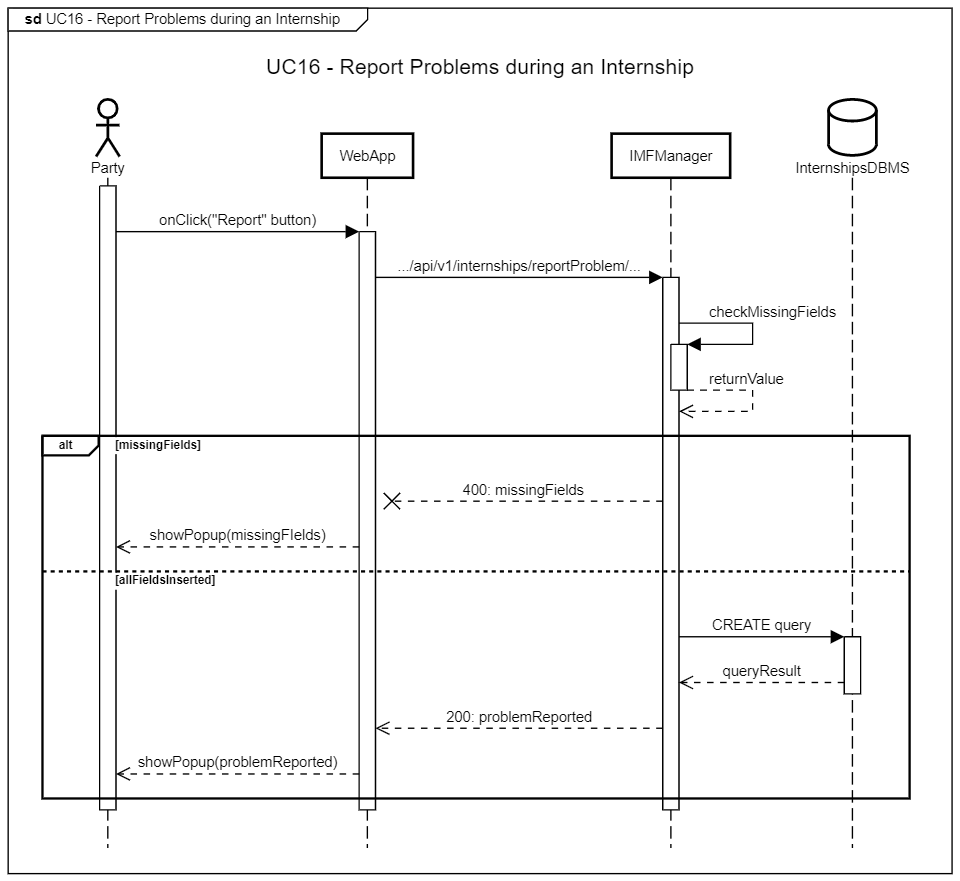
\includegraphics[width=1\linewidth]{LaTeXCode/images/SequenceDiagrams/UC16-sequenceDiagram.png}
         \caption{Report Problems during an Internship}
         \label{fig:report_problems_sd}
     \end{center}
\end{figure}

\newpage

\subsubsection*{SD\cuc. Handle Problems during an Internship}
\label{subsubsec:handle_problems_sd}
The University initiates the process by clicking one of the "Mark as In Progress", "Mark as Solved" or "Hide" buttons on a problem's widget in its dashboard page, triggering a request to the \texttt{.../api/v1/internships/handleProblem/...} API endpoint, managed by the \texttt{IMFManager}. The \texttt{IMFManager} updates the problem's status in the \texttt{InternshipsDBMS} according to the button clicked by the University. Upon successful completion, the \texttt{WebApp} receives confirmation and notifies the University with a popup indicating that the problem has been correctly marked as solved.

\begin{figure}[H]
    \begin{center}
         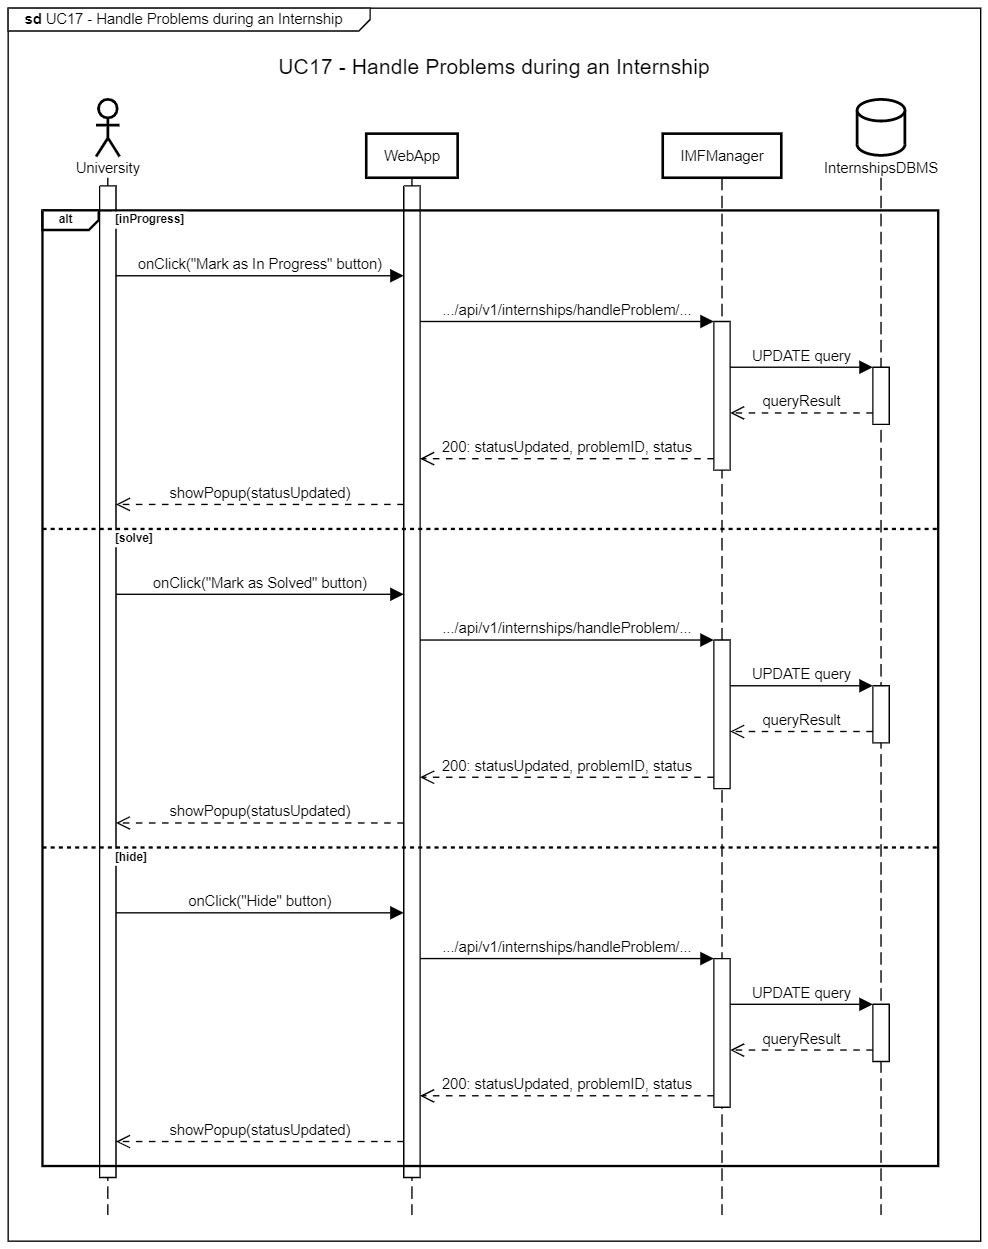
\includegraphics[width=0.75\linewidth]{LaTeXCode/images/SequenceDiagrams/UC17-sequenceDiagram.png}
         \caption{Handle Problems during an Internship}
         \label{fig:handle_problems_sd}
     \end{center}
\end{figure}

\newpage

\subsubsection*{SD\cuc. Report Feedback after an Internship}
\label{subsubsec:report_feedback_sd}
The Party begins by clicking the "Submit" button in the widget of an ended internship on their dashboard page, sending a request to the \texttt{.../api/v1/internships/reportFeedback/...} API handled by the \texttt{IMFManager}, which processes the request and updates the relevant records in the \texttt{InternshipsDBMS}. Once the feedback is successfully recorded, the \texttt{WebApp} is notified of the successful operation and displays a confirmation popup to the Party.

\begin{figure}[H]
    \begin{center}
         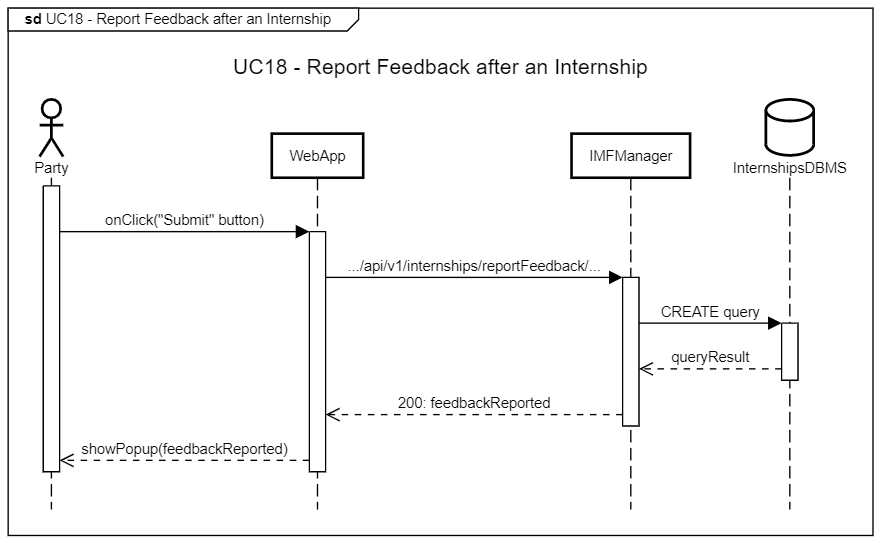
\includegraphics[width=1\linewidth]{LaTeXCode/images/SequenceDiagrams/UC18-sequenceDiagram.png}
         \caption{Report Feedback after an Internship}
         \label{fig:report_feedback_sd}
     \end{center}
\end{figure}

\newpage

\subsubsection*{SD\cuc. Suggest Optimizations for a Student Profile}
\label{subsubsec:suggest_optimizations_student_sd}
The Student initiates the action by clicking the "Improve Profile" button on their profile page, triggering a request to the \texttt{.../api/v1/optimizations/optimizeStudent/...} API endpoint, which is managed by the \texttt{OptimizationManager}. The \texttt{OptimizationManager} retrieves relevant data from the \texttt{RecommendationsDBMS} and processes the information to generate optimization suggestions. Once completed, the \texttt{OptimizationManager} sends the suggestions back to the \texttt{WebApp}, which displays them to the student.

\begin{figure}[H]
    \begin{center}
         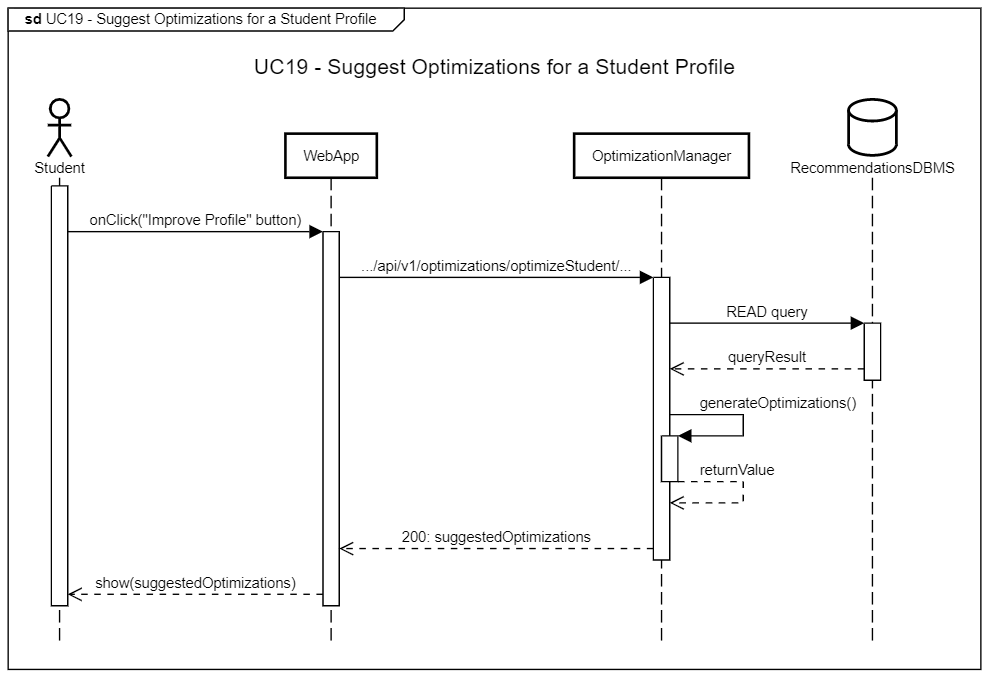
\includegraphics[width=1\linewidth]{LaTeXCode/images/SequenceDiagrams/UC19-sequenceDiagram.png}
         \caption{Suggest Optimizations for a Student Profile}
         \label{fig:suggest_optimizations_student_sd}
     \end{center}
\end{figure}

\newpage

\subsubsection*{SD\cuc. Suggest Optimizations for an Internship Offer}
\label{subsubsec:suggest_optimizations_internship_sd}
This Sequence Diagram is the same as the previous one, with the only difference being that it is started by a Company and not by a Student, and thus is about optimizing an offer and not a profile.

\begin{figure}[H]
    \begin{center}
         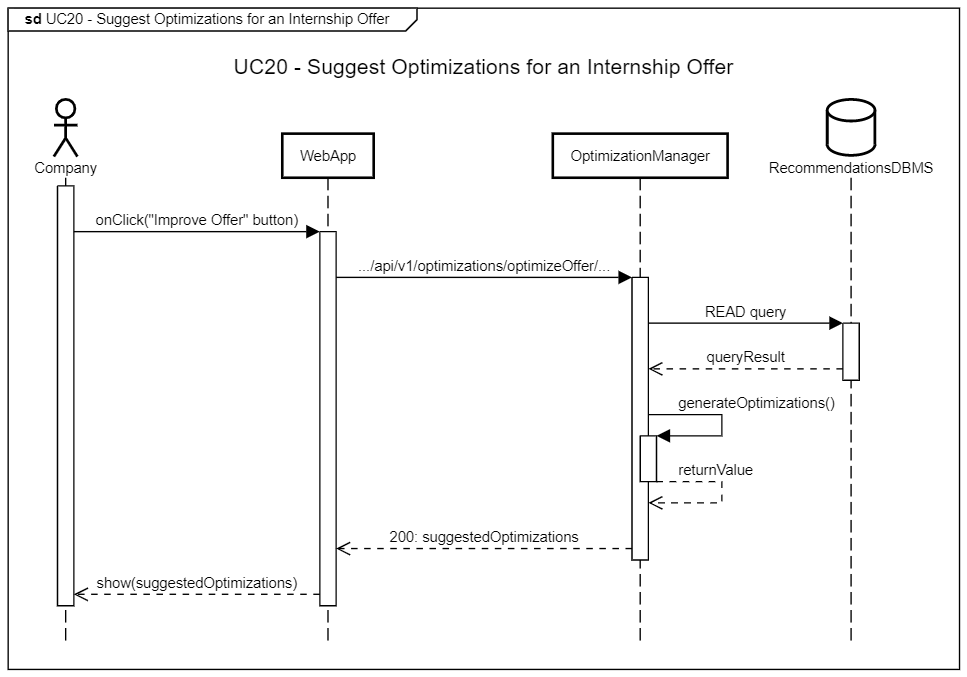
\includegraphics[width=1\linewidth]{LaTeXCode/images/SequenceDiagrams/UC20-sequenceDiagram.png}
         \caption{Suggest Optimizations for an Internship Offer}
         \label{fig:suggest_optimizations_internship_sd}
     \end{center}
\end{figure}

\newpage

\section{Selected Architectural Styles and Patterns}
\label{sec: patterns}%

For the S\&C system, various styles and patterns allow for better management of the key aspects of the system:

\begin{itemize}
    \item \textbf{Database-per-service pattern:} When implementing a system as a microservices architecture, it is strongly advised to partition the domain data according to the bounded contexts identified, obtaining one separate database for each service \hyperref[document: cloud_native_data_patters]{[3]}. This pattern comes with many advantages: independent scalability between the services, localized impact of schema evolutions or failures, and the possibility of using different technologies for distinct databases according to the needs of the specific domains. As a consequence, multiple databases are present in the S\&C system: the SecurityDB, the ProfilesDB, the InternshipsDB and the RecommendationsDB: for instance, if one of these databases goes down, the other microservices are not impacted at all.

    \item \textbf{Functional partitioning:} As just stated, data is partitioned among the various databases according to the bounded context of each microservice: in order to reduce cross-service queries to the bare minimum, bounded contexts have been identified as the different macro-functionalities that the system is required to offer, therefore adhering to a functional partitioning model \hyperref[document: data_partitioning]{[4]}. However, monitoring of the workload and distribution of data across all the databases should be constantly monitored, so that the database architecture can be redesigned as needed by performance issues, for example by adding horizontal partitioning (sharding) to the partitioning already in place.
    
    \item \textbf{Eventual consistency:} As the (in)famous CAP theorem states, it is impossible for a distributed system to achieve consistency, availability and partition tolerance (CAP) all at the same time \hyperref[document: relational_nosql_data]{[5]}. Given the choice of structuring the S\&C platform as a distributed system and the somewhat strict requirements on availability outlined in Section 3.5.2 \textit{Availability} of the RASD, the system is designed to be available and partition-tolerant alone, settling on only the eventual consistency of data across the spread-out databases and replicas. As the S\&C application is not handling critical processes, eventual consistency isn't really a problem \hyperref[document: data_consistency]{[6]}, as it doesn't matter if information about any offer isn't immediately up-to-date, or if a recommendation is not generated instantly after a new offer becomes available, or if some recommendations do not take into account the absolute latest information available.

    \item \textbf{Event Sourcing pattern:} A common choice to achieve data replication across a cluster of databases is implementing an event-driven architecture, also known as publish-subscribe: changes in the data one of the replicas generate events that get sent to all the other replicas. As stated before, tools based on the Raft protocol might be helpful: an example of such tools is Apache Kafka, which can be used as a channel to share the events between all the database copies. Kafka also supports multiple topics, enabling replication for different clusters of databases at the same time, and can also be configured to guarantee exactly-once semantics for ensuring events are not duplicated. Moreover, additionally to standard data replication, keeping data semantically separated comes with a cost, as some data is to be replicated across the different databases: this is the case for the RecommendationsDB, which is meant to gather data from the ProfilesDB and from the InternshipDB, representing something similar to what is called a \textbf{Materialized View}. As this can also be seen as a form of data replication, the standard Kafka distribution can also help: however, given that the involved databases are implemented with heterogeneous technologies, another suitable choice is to employ Kafka Connect with Change Data Capture (CDC), detecting changes in the databases by defining source connectors on the ProfilesDB and on the InternshipsDB and replicating them through a sink connector on the RecommendationsDB.

    \item \textbf{API Gateway pattern:} By introducing this pattern, the system establishes a single entry point for all client requests, unifying interactions with other components. Using NGINX, the system manages request routing to microservices and performs URL rewriting for necessary redirections. This approach enhances security by exposing only one public endpoint and optimizes internal traffic management. The benefits of adopting this pattern in our system include isolating clients from the internal partitioning of microservices, shielding them from the complexity of determining service instance locations, reducing the number of requests, and simplifying the client by shifting the logic for interacting with multiple services to the API Gateway \hyperref[document: api_gateway]{[7]}.

    \item \textbf{Circuit Breaker pattern:} In order for graceful degradation of the system to be completely achieved, it is necessary to take full advantage of the microservices architecture by implementing the Circuit Breaker pattern in the API Gateway directing the communications. In this way, microservices don't block or suffer from other services' slowdowns or failures, as the "link" between them can be opened and closed at will according to their current status, so that each service can keep functioning and offering limited functionalities also when it isn't able to make requests to another one.
\end{itemize}